\documentclass[UKenglish]{ifimaster}  %% ... or USenglish or norsk
\usepackage[utf8]{inputenc}           %% ... or latin1
\usepackage[T1]{fontenc,url}
\urlstyle{sf}
\usepackage{babel,textcomp,csquotes,duomasterforside,varioref,graphicx}
\usepackage[backend=biber,style=numeric-comp]{biblatex}
\usepackage{amsmath,amssymb,amsfonts}
\usepackage{algorithmic}
\usepackage{textcomp}
\usepackage{xcolor}
\usepackage{textgreek}
\usepackage{float}
\usepackage{graphicx}
\usepackage{chemformula}
\usepackage{cleveref}
\usepackage{caption}
\usepackage{subcaption}
\usepackage{booktabs}

\raggedbottom %%reduces the gaps between the paragraphs

\title{Thesis Title}        %% ... or whatever
\subtitle{A subtitle of your thesis }         %% ... if any
\author{Author name}                      %% ... or whoever 

\addbibresource{bibliography.bib}            %% ... or whatever
\graphicspath{{figures/}}
\DeclareUnicodeCharacter{2212}{-}
\includeonly
{
	%chapter/chapter_background,
    %chapter/chapter_2,
    %chapter/chapter_3,
    %chapter/chapter_4,
    %chapter/chapter_5,
    %chapter/chapter_6,
    chapter/chapter_7
}


\begin{document}
\duoforside[dept={Department Name <change at main.tex>},   %% ... or your department
  program={Master's Program Name <change at main.tex>},  %% ... or your programme
  long]                                        %% ... or long

\frontmatter{}  
\chapter*{Abstract}                   %% ... or Sammendrag or Samandrag

\tableofcontents{}
\listoffigures{}
\listoftables{}

\chapter*{Preface}                    %% ... or Forord

\mainmatter{}

\chapter{Introduction}                  %% ... or Bakgrunn

\textbf{some introduction on the importance of discovering new materials and alloying}.\\

High-entropy alloys is a novel class of materials based on alloying multiple components, as opposed to the more traditional binary alloys. This results in an unprecedented opportunity for discovery of new materials with a superior degree of tuning for specific properties and applications. Recent research on high-entropy alloys have resulted in materials with exceedingly strong mechanical properties such as strength, corrosion and temperature resistance, etc \textbf{find references}. Meanwhile, the functional properties of high-entropy alloys is vastly unexplored. In this study, we attempt to broaden the knowledge of this field, the precise formulation of this thesis would be an exploration on the possibilities of semiconducting high-entropy alloys. 

A key motivation of this thesis is the ability to perform such a broad study of complex materials in light of the advances in material informatics and computational methods. In this project, we will employ Ab initio methods backed by density functional theory on top-of the line supercomputers and software. 20 years ago, at the breaking point of these methods, this study would have been significantly narrower and less detailed firstly, but secondly would have totaled ... amount of CPU hours to complete (\textbf{Calculate this number}). In the addition to the development in computational power, is also the progress of modeling materials, specifically we will apply a method called Special Quasi-random Structures (SQS) to model high-entropy alloys or generally computationally complex structures. Together with the open landscape of high-entropy alloys described above, these factors produce a relevant study in the direction of applying modern computational methods to progress the research of a novel material class and indicate promising directions within the field.   
 
In specifics, this thesis revolve around the electrical properties of high-entropy alloys, mainly the band gap as this is the key indicator for a semiconducting material and it's applicability. Semiconductors are the building blocks in many different applications in today's world, ranging from  optical and electrical devices, to renewable energy sources such as solar and thermoelectricity. Given the economic and sustainable factors concerning silicon, in addition to its role in relevant applications such as microelectronics and solar power. Silicon emerges as a natural selection to build our alloys around. Furthermore, the development and research on both high entropy alloys and metal silcides have been heavily centered around 3d transition metals. Keeping in line with the economic and environmental factors, we will continue this direction by focusing on high entropy stabilized sustainable and economic 3d metal silicides \textbf{Not happy with this writing}. Throughout the study we will analyze a great number of permutations of 3d silicides, from different initial metal silicides such as $CrSi_2, FeSi_2, MnSi_{1.75}, Fe_2Si$, each with distinct properties relating to the band gap, crystal structure and metal to silicon ratio. In addition, the permutations include numerous metal distributions and elements within the 3d-group of metals. Examples are Co, Cr, Fe, Mn, and Ni. 

Given a background in high-entropy alloys, one could ask if this study is truly sensible. In the later sections we will cover the details of this field, and it quickly become clear that the materials investigated in this study does not fall under the precise definition of high-entropy alloys, nor do we intend to explore the properties and factors relating to high-entropy stabilized alloys such as the configurational entropy, phase stability and finite temperature studies. However this study is motivated from the discovery of these materials and promising properties, and venture into a more hypothetical space of materials, enabled by the computational methods available to study the potential properties of such materials. On the other hand, very recent studies \textbf{Mari, and other HEA silicide study} have experimentally produced high-entropy disilicides, thus in some way justifying the direction of this project. 

We begin this project by reviewing key concepts of solid-state physics for readers lacking a background in materials science, and an introduction to the base 3d silicides of the experimental work. Later follows a theoretic walk-through of the relevant concepts of this thesis, these topics include high-entropy alloys, special quasi-random structures, and density functional theory. Next we shine light on the implementation of DFT in this project, and other computational details required to reproduce the results in this thesis, such as the use of the Vienna Ab Initio Simulation Package (VASP) and implementation of SQS. Finally we present the results of our study, these include the band gap and electronic properties of various structures and the success and challenges of the computational methods applied throughout the study. 

\part{Theory}                    %% ... or ??
\chapter{Background}
\label{sec:background}

\section{Solid-state physics}
\textbf{Contents are band-theory, dos, reciprocal space, BZ}

\section{Silicides}
\textbf{This section should contain a brief overview of the silicides used in this project, ie crystal structure and electronic properties of Fe2Si, FeSi2, MnSi175, CrSi2}
\chapter{High-Entropy alloys}
\label{sec:HEA}

High-Entropy Alloys (HEAs) has become an increasingly popular field in materials science, due to the large flexibility and possibilities for discovery of new materials with unique properties. Since the staring point of high-entropy alloys in 2004, as of 2015 there has been over 1000 published journal articles on high-entropy alloys \cite{hea2016_ch1}. In the following section we will cover the fundamentals and some applications of high-entropy alloys. This section is based on the fantastic description of HEAs in the book "High-Entropy Alloys - Fundamentals and Application", in particular chapters 1,2,3 and 7 \cite{hea2016_ch1}, \cite{hea2016_ch2}, \cite{hea2016_ch3}, \cite{hea2016_ch7}, and references therein.

\section{Fundamentals} 
A high entropy alloy can in a way be compared to a smoothie. In a smoothie one can produce unique combinations of flavors and nutritional values based on both the properties of the individual fruits and vegetables, and their interplay in the mixture. In materials science, a similar approach can be applied to generate a large range of materials with tunable properties depending on the intended application. In respect to HEAs, examples can be increased strength, ductility, corrosive resistance and low thermal conductivity. Moving on from the rather banal fruit analogy, a high-entropy alloy can be defined from two conditions:
\begin{enumerate}
    \item The material consists of at least 5 distinct elements, where each element contribute between 5-35$\%$ of the composition.
    \item The total configurational entropy is greater than 1.5R, where R is the gas constant. 
\end{enumerate}
The latter is an especial case for high-entropy alloys. The ideal configurational entropy of a random N-component solid-solution is described as
\begin{equation}
\Delta S_{\text{config}} = -R \sum_{i=1}^{N}X_i\ln X_i,
\end{equation}
where $X_i$ is the mole fraction of the $i$th component. Its clear that $\Delta S_{\text{config}}$ increase with a higher number of constituents in the mix. For instance, the ideal configurational entropy of a equimolar binary alloy is 0.69 R, as opposed to 1.61 R in a five-component equimolar alloy. If we neglect the other factors that influence the formation of solid solutions (will be covered later), from Gibbs free energy
\begin{equation}
\Delta G_{\text{mix}} = \Delta H_{\text{mix}} - T\Delta S_{\text{mix}},
\end{equation} 
the two primary factors in formation of solid solution are the mixing enthalpy, which is the driving force to form compounds, and the mixing entropy which is the driving force to form random solid solutions. At elevated temperatures especially, the energy associated to the entropy of the system becomes comparative to the mixing enthalpy and can impact the formation. In summary, the overall concept of high-entropy alloys is that through alloying a greater number of elements, the gain in configurational entropy of the system prohibits the formation of intermetallic compounds, in favor of random solid solution. The random term simply relate to the various components occupying lattice positions based on probability. In fact, a narrower definition of high-entropy alloys would be structures with a single-phase disordered solid solution. The two "definitions" given previously, can be considered as guidelines for the latter.
 
Although the mixing entropy mentioned above plays a central role in the formation, there are other factors to consider that can either favor or oppose the formation of a single disordered phase. One of these is the atomic size effect, which is related to the differences in atomic size between constituents in the alloy. This quantity is denoted $\delta$. Y. Zhang et al. in 2008 illustrated the relationship between $\Delta H_\text{mix}$ and $\delta$. When $\delta$ is very small, in other words when the alloys are comprised of elements with similar atomic sizes, the elements have an equal probability to occupy lattice sites to form solid solutions, but the mixing enthalpy is not negative enough to promote formation of solid solution. Increasing $\delta$ results in greater $\Delta H_\text{mix}$, but leads to a higher degree of ordering. The formation of solid solution high-entropy alloys occur in a narrow range of $\delta$ values, that satisfy both the enthalpy of mixing and the disordered state. Recently, Yang and Zhang proposed the parameter $\Omega$ to evaluate the stability of high-entropy alloys. This quantity is a product of the melting temperature $T_m$, mixing entropy and mixing enthalpy in the following relation

\begin{equation}
\Omega = \frac{T_\text{m} \delta S_\text{mix}}{|\Delta H_\text{mix}|}.
\end{equation}

They found that the formation of single disordered solid solution occurs at $\Omega \geq 1.1$ and $\delta \leq 6.6\%$, while compounds such as intermetallics form for greater values of $\delta$ and lesser values of $\Omega$. Similarly, replacing the atomic size effect with the number of elements results in an equivalent condition. These findings are summarized in figure 2.1.
\begin{figure}[H]
\centering
\begin{subfigure}{.85\textwidth}
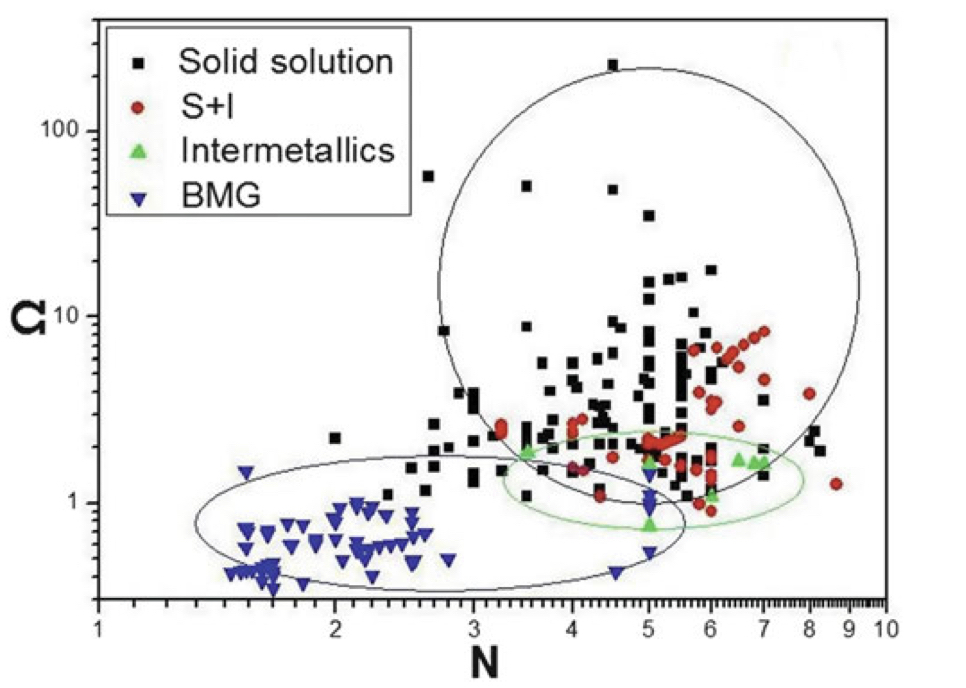
\includegraphics[width=\textwidth]{theory/heaformation1.jpeg}
\caption{HEA formation based on $\Omega$ and the atomic size effect $\delta$}
\end{subfigure}
\begin{subfigure}{.85\textwidth}
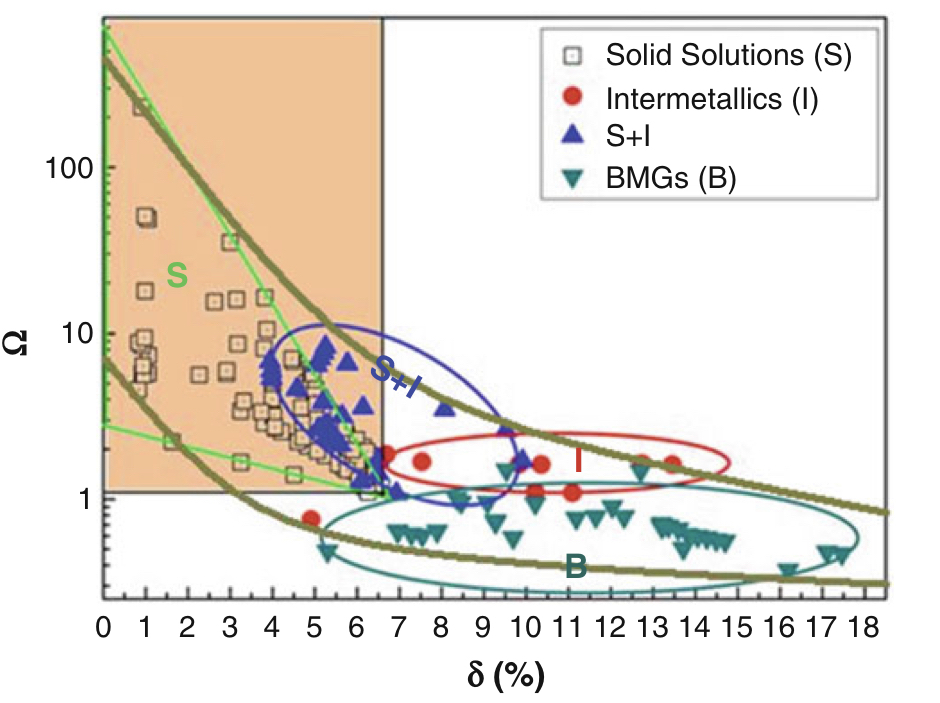
\includegraphics[width=\textwidth]{theory/heaformation2.jpeg}
\caption{HEA formation based on $\Omega$ and the number of consituents $N$}
\end{subfigure}
\caption{Formation of HEAs based on $\Omega = \frac{T_\text{m} \delta S_\text{mix}}{|\Delta H_\text{mix}|}.$, the atomic size effect $\delta$, and number of constituents $N$. Figures adopted from \cite{hea2016_ch2}}
\end{figure} 
An important quantity in terms of characterizing high-entropy alloys, is the total number of valence electrons VEC. Derived from the work of Guo et al. on the phase stability of the \ch{Al_xCrCuFeNi_2} HEA, the VEC can be directly related to the crystal structure of high-entropy alloys. A lower VEC stabilize the BCC phase, while higher values stabilize FCC, in between is a mixture of the two. Specifically values greater than 8.0 stabilize FCC, and values bellow 6.87 favor BCC. However, these boundaries are not rigid when including elements outside of transition metals, exceptions has also been found for high-entropy alloys consisting of manganese. Although a heavy majority of reported high-entropy alloys that form solid solutions has been found to adopt simple cubic structures, such as FCC and BCC. In addition to the high-entropy silicides mentioned in the introduction, recent studies has reported HEAs in less symmetric structures, such as \ch{CoFeMnTi_x V_y Zr_z}, \ch{CrFeNiTiVZr} and \ch{CoFeNiTi} in HCP, as well as the \ch{Ti_{35}Zr_{27.5}Hf_{27.5}Ta_5Nb_5} HEA in the orthorhombic crystal system.  

\section{Core effects and properties}
In this section, we will summarize the discussion above into four core effects that can be used to explain high entropy alloys, and discuss some of the properties observed in various HEAs. The first core effect is called the "high-entropy effect", as explained in the previous section the high configurational entropy of HEAs compared to traditional solids or even binary alloys is central to stabilize the disordered phase ahead of intermetalic or strongly ordered structures. This effect can result in enhanced strength and ductility. From considerations of Gibbs free energy, we see that this effect is most prominent at elevated temperatures.

The second effect is the "severe lattice distortion effect" that arises from the fact that every element in a high-entropy structure is surrounded by non-homogeneous elements, thus leading to severe lattice strain and stress. The overall lattice distortion is additionally attributed to the differences in atomic size, bonding energies and crystal structure tendencies between the components. Therefore, the total lattice distortion observed in HEAs are significantly greater than that of conventional alloys. This effect mostly affects the strength and conductivity of the material, such that a higher degree of distortion yields greater strength and greatly reduces the electronic and thermal conductivity due to increased electron and phonon scattering. An upside to this is that the scattering and following properties become less temperature dependent given that it originates from the lattice rather than thermal vibrations. The concept of lattice strain in high-entropy alloys can be visualized as in figure 2.2.

\begin{figure} 
\centering
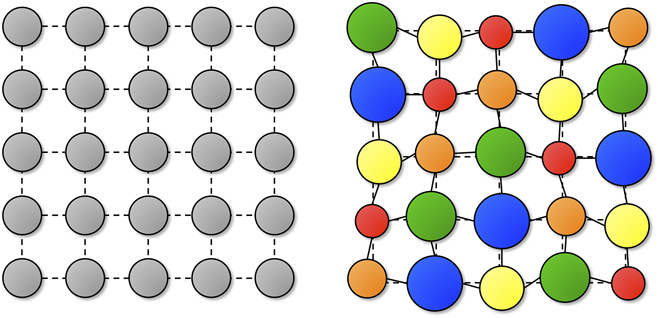
\includegraphics[width=\textwidth]{theory/latticeDistortionHEA.jpeg}
\caption{A schematic illustration of lattice distortion in high-entropy alloys, compared to conventional materials. Figure from \cite{owen_jones_2018}.}
\end{figure}
 
The two remaining effects, "sluggish diffusion" and "cocktail effect" can be summarized swiftly. The first is a direct consequence of the multi-component layout of high-entropy alloys that results in slowed diffusion and phase transformation because of the number of different elements that is involved in the process. The most notable product from this effect is an increased creep resistance. Lastly, we have the cocktail effect which is identical to the smoothie analogy mentioned previously, in that the resultant characteristics of a high-entropy alloy is a combination of both the individual elements and their interplay. This is possible the most promising concept behind high-entropy alloys, which fuels researchers with ambitions to discover highly optimized materials by meticulously combining and predicting properties from different elements. Examples of this can be the refractory HEAs developed by the "Air Force Research Laboratory" that significantly exceeded the melting points and strength of previous Ni or Co-based superalloys, by alloying specifically refractory elements such as Mo. Nb and W. Another example is the research conducted by Zhang et al. on the high-entropy system \ch{FeCoNi(AlSi_x)}, with ($0 < x 0.8$). In this HEA it was found that increased amount of either Al or Si lowered the saturation magnetization of the alloy. By tuning the relative amounts, it was found excellent properties for an $x=0.2$ HEA in terms of the magnetization, electrical resistivity and yield strength to produce a promising soft-magnet. The same was also found in \ch{Al_{0-2}CoCrFeNi} HEAS, where the addition of Al reduced the ferromagnetism of the alloy, and in \ch{CoCrCuFeNiTi_x} alloys where $x = 0$ was paramagnetic and $x > 0.8$ showed superparamagnetic properties. In general we find that that the saturation magnetism is mostly dependent on the contents and distribution of ferromagnetic elements such as Fe, Co and Ni while the addition of anti-ferromagnets like Cr could be difficult to predict. For example in the ferromagnetic HEA CoFeMnNiX, X = Al, Cr, Ga, Sn, studied in \cite{ZUO201710}, Mn pushed the material to the ferromagnetic phase, meanwhile addition of Cr pushed the material to a paramagnetic phase. Likewise in the equimolar system of \ch{CrMnFeCoNi} \cite{PhysRevB.96.014437}, the local magnetic moment of Cr was found to align antiferromagnetic, and the ferromagnetic character was attributed to local magnetic moments around Fe and Mn. 

As we have seen from the above examples, what makes high-entropy alloys a particularly interesting and promising field, is that they possesses the ability to be tuned for specific applications and properties, by testing specific combinations and distributions of different elements. In many ways, not indifferent to a smoothie or a cocktail.
\chapter{Density-Functional Theory}
\label{sec:label3}


\section{dft}


\chapter{Density-Functional Theory}
\label{sec:DFT}

\section{Review of Quantum Mechanics}

\subsection{The Shr\"{o}dinger equation}
The Schr\"{o}dinger equation composed of the wavefunction $\Psi(\vec{r},t)$ and Hamiltonian $\hat{H}(\vec{r},t)$ where $\vec{r}$ and $t$ is the spatial position and time respectfully.
\begin{equation}
    i\hbar\frac{\partial}{\partial t}\Psi(\vec{r}, t) = \hat{H}(\vec{r},t)\Psi(\vec{r}, t)
\end{equation}
The time-independent shr\"{0}dinger equation for the eigenvalues $E_k$ of the $k$-th eigenvalue $\psi_k(\vec{r}$
\begin{equation}
    \hat{H}\psi_k(\vec{r}) = E_k \psi_k(\vec{r})
\end{equation}
Extending to a system comprised of multiple particles, we have the many-particle Shr\"{o}dinger equation, involving the many-body Hamiltonian. This quantity is composed of the kinetic energy of $N_e$ electrons $T_e$, the interaction energy between electrons $U_{ee}$, the kinetic energy of $N_n$ nuclei, the coulomb interaction between nuclei $U_{nn}$, and finally the attractive interaction between nuclei and electrons $U_{en}$. In the equation bellow for the may-body equation, we use the following symbols and notation: $m_e$ = electron mass, $m_n$ = nuclei mass, $\epsilon_0$ = permittivity in vacuum, $q$ = particle charge, $\alpha$ = nuclei number, $Z_a$ = atom number of nuclei $\alpha$, $r$ = position of electron, $R$ = position of nuclei.
\begin{align}
    \hat{H} &= T_e + T_n + U_{ee} + U_{nn} + U_{en} \\
    \begin{split}
        &= -\sum_{j=1}^{N_e}\frac{\hbar^2\nabla_j}{2m_e} - \sum_{\alpha=1}^{N_n}\frac{\hbar^2 \nabla_\alpha}{2m_n} + \frac{1}{4\pi \epsilon_0}\sum_{j=1}^{N_e}\sum_{j'<j}\frac{q^2}{|r_j - r_{j'}|} \\
    &+ \frac{1}{4\pi\epsilon_0}\sum_{\alpha=1}^{N_n}\sum_{\alpha' < \alpha}\frac{q^2Z_\alpha Z_{\alpha'}}{R_\alpha - R_{\alpha'}} - \frac{1}{4\pi\epsilon_0}\sum_{j=1}^{N_e}\sum_{\alpha=1}^{N_n}\frac{q^2Z_\alpha}{|r_j - R_\alpha|}
    \end{split}
\end{align} 

\subsection{Simplifications and approximations to solve the many-electron Shr\"{o}dinger equation}

\subsubsection{Born-Oppenheimer}
Challenges with solving many-particle Shr\"{o}dinger equation is i) computationally expensive, ii) need to know how $\Psi$ depends on single particle wavefunctions $\psi_k$. To solve this complex problem, we need approximations. Particularly Born-Oppenheimer and Harte-Fock approximations. The first makes the cleaver and reasonable assumption that since the electron mass is negligibly small in comparison to that of a nuclei, we can treat the nuclei as point charges, enabling us to divide the eigenfunction into a separate electronic and nuclear part, ie
\begin{equation}
    \Psi_{k}^{en}(\vec{r}, \vec{R}) \approx \Psi_k(\vec{r}, \vec{R}) \Theta_k(\vec{R})
\end{equation}
where we have written the complete wavefunction in terms of an electronic part $\Psi_k(\vec{r}, \vec{R})$ and nuclear part $\Theta_k(\vec{R})$. The dependencies come from the fact that electrons can respond instantaneously to new positions of the nuclei, therefore the $\vec{R}$ dependence. Writing this in terms of the Hamiltonian we get
\begin{align}
    &\left( T_{e} + U_{ee} + U_{en} \right) \Psi_k(\vec{r}, \vec{R}) = E_k(\vec{R})\Psi_k(\vec{r}, \vec{R}) \\
    &\left( T_{n} + U_{nn} + E_k(\vec{R}) \right) \Theta(\vec{R}) = E_{k}^{en}(\vec{R})\Theta_k(\vec{r}, \vec{R}).
\end{align}
The two sections are interrelated through the electronic energy eigenvalue $E_k(\vec{R})$. Furthermore, the left hand side of the nuclear part can be simplified to $U_{nn} + E_k(\vec{R})$, assuming that the kinetic energy of point charges is zero. This simplified expression for the nuclear left hand side is called for the potential energy surface (EPS).

\subsubsection{Hartree-Fock}
The next step in line is to find a wavefunction that can describe all electrons in a system. This was originally done by Hartree, which assumed that electrons can be described independently and suggested the ansatz for a two-electron wavefunction
\begin{equation}
    \Psi_k(\vec{r_1}, \vec{r_2}) = A \cdot \psi_1(\vec{r_1}) \psi_2(\vec{r_2}),
\end{equation}
where A is the normalization constant. However this approximation does not account for the fact that electrons are indistinguishable and hence does not obey the Pauli exclusion principle for ferminons. This was overcome with the Hartree-Fock approximation that implement an anti-symmetric wavefunction. The full expression is given bellow
\begin{equation}
    \Psi_k(\vec{r_1}, \vec{r_2}) = \frac{1}{\sqrt{2}} \Big( \psi_1(\vec{r_1}) \psi_2(\vec{r_2}) - \psi_1(\vec{r_2})\psi_2(\vec{r_1}) \Big)
\end{equation}

The Hartree-Fock (HF) approximation makes the electrons distinguishable and hence obey the Pauli exclusion principle, this means that the exchange energy is accounted for. On the other side, HF is not a complete description as it fails to model the electron correlations. 

\subsubsection{The Variational principle}
In materials science, the overarching concern is the ground-state properties of a system. This can be found efficiently and easy by whats known as the variational principle. This states that the energy of any trial wavefunction will always be higher than the ground-state energy $E_0$, ie
\begin{equation}
    E_0 = \langle\psi_0|H|\psi_0\rangle \leq \langle\psi|H|\psi\rangle = E
\end{equation}
This enable us to find the ground state energy and corresponding wavefunction by a minimization technique. Next, we will present the basics of the density functional theory for how these equations can be solved numerically and efficiently in order to study real materials and systems.

\section{Fundamentals of Density-Functional Theory}
The density functional theory was developed by Hohenberg and Kohn in 1964 and revolved around the fact that the ground-state density can be expressed in terms of the ground-state wavefunction. We have
\begin{equation}
    n_0(r) = |\Psi_0(r)|,
\end{equation}
furthermore the theorem states that all ground-state physical properties can be found as unique functionals of the ground-state density. The biggest upside of this, is that instead of trying to solve the many-body Shr\"{o}dinger equation to obtain the ground-state wavefunction, we have reduced the computational complexity from $3N_e$ to $3$. Thus, the Hohenberg and Kohn density functional theory makes for a promising and effective method to obtain the ground-state properties of a system, given that the exact electron density functional is known. However, this is still 60 years later unknown. 

The density functional theory build on two specific theories, called the Hohenberg-Kohn theorems. They are:
\begin{enumerate}
    \item For any system of interacting particles in an external potential $V_{ext}$, the density is uniquely determined.
    \item There exists a variational principle for the energy density functional such that, if $n$ is not the electron density of the ground-state, them $E[n_0] < E[n]$.
\end{enumerate}
The proof behind both theorems can be found in appendix .. A direct result of the second theorem is the energy can be described as a function of the density
\begin{equation}
    E[n] = T[n] + U_{ee}[n] + U_{en}[n],
\end{equation}
where the first two terms $T[n]$ and $U_{ee}[n]$ make up the Hohenberg-Kohn functional. 

We know move on to the Kohn-Sham equations, in which Kohn and Sham expressed the exact ground-state density from Hartree type wavefunctions. 
\begin{equation}
    \Psi(\vec{r}_1, \vec{r}_2 , .., \vec{r}{N_e}) = \psi_1^{KS}(\vec{r}_1)\psi_2^{KS}(\vec{r}_2)...\psi_{N_e}^{KS}(\vec{r}_{N_e})
\end{equation}
In which, $\psi_j^{KS}$ are auxiliary independent single-particle wavefunctions. We know modify the equation for total energy as a function of density defined by the second theorem, to include the single auxiliary wavefunctions and their corresponding kinetic energy and interaction energy. We get:
\begin{equation}
    E[n] = T_s[n] + U_s[n] + U_{en}[n] + (T[n] - T_s[n]) + (U_{ee}[n] - U_s[n]).
\end{equation}
with the s subscript denoting the single particle wavefunctions. The latter two terms are known as the exchange-correlation energy $E_{xc}$
\begin{equation}
    E_{xc}[n] = \Delta T + \Delta U
\end{equation}

This term is responsible for the many-electron interaction. The complete total energy functional can now be expressed as
\begin{equation}
    \begin{split}
    E[n] &= \overbrace{\sum_j \int \psi_j^{KS*}\frac{-\hbar^2 \nabla^2}{2m}\psi_j^{KS}d\vec{r}}^{T_s[n]} + \overbrace{\frac{1}{2}\frac{1}{4\pi \epsilon_0} \int \int q^2 \frac{n(\vec{r})n(\vec{r}')}{|\vec{r} - \vec{r}'|}d\vec{r}\vec{r}'}^{U_s[n]} \\ 
        &+ \underbrace{\int V_{en}(\vec{r}n(\vec{r})d\vec{r}}_{U_en[n]} + \underbrace{(T[n] - T_s[n]) + (U_{ee}[n] - U_s[n])}_{E_{xc}[n]}
    \end{split}
\end{equation}

Finally we write the complete expression for the Kohn-Sham single-electron equations given an exact exchange-correlation energy and utilizing the variational principle described previously
\begin{equation}
    \bigg\{ -\frac{\hbar^2}{2m_e}\nabla^2_s + v_H(\vec{r}) + V_{en}(\vec{r}) + V_{xc}(\vec{r} \bigg\}\psi_s^{KS}(\vec{r}) = \epsilon_s^{KS}(\vec{r})\psi_s^{KS}(\vec{r}),
\end{equation}
Define $V_H$, and $V_{xc}$ and mention that the former include self interaction that can be accounted for in XC functional. Finally, the total energy of the many-electron system is defined as
\begin{equation}
    E[n] = \sum_j \epsilon_j^{KS} - \frac{1}{2}\frac{1}{4\pi\epsilon_0} \int \int q^2 \frac{n(\vec{r})n(\vec{r}')}{|\vec{r} - \vec{r}'|}d\vec{r}d\vec{r}' + E_{xc}[n] - \int V_{xc}(\vec{r})n(\vec{r})d\vec{r}.
\end{equation}
This is the fundamental working principle of the density functional theory and Kohn-Sham equations.

\section{Limitations of DFT}
\begin{itemize}
    \item Local minima method
    \item Not exact $V_{xc}$, means we must compromise between accuracy and cost, and choose between the different methods for specific application. There is no one best overall method that is superior for all purposes. 
    \item Not exact kohn-sham eigenfunctions
    \item Band gap
\end{itemize}



\part{Methodology and Implementation}
\chapter{Material}
\label{sec:label5}


\section{Something}


\chapter{Computational details}
\label{sec:Computation}

This section is intended to provide the necessary details for reproduction of results to be presented later on. First we begin by describing the software used for the project. 

\section{Vienna Ab initio Simulation Package}
This software, often referred to as VASP is a package for ab initio quantum mechanics calculations using the projected augmented wave method and plane wave basis set. The intended methodology is DFT, but have been extended for methods post the original DFT-formulation. Calculations with VASP was carried out on the supercomputer fram, with allocated time and resources provided by Uninett Sigma2,\textbf{add reference!}.

The structure of VASP rely on a set of input files and output files from the calculation, the input files required to perform a DFT computation in VASP are the following:
\begin{itemize}
    \item INCAR - this file provide the tags responsible for different methods, algorithms, parameters etc.
    \item POSCAR - this file is related to the crystal structure of the system
    \item POTCAR - What psudopotential that is used
    \item KPOINTS - A file containing information on what KPOINTS will be used
    \item jobfile - This file contains information for the supercomputer regarding resources and such.
\end{itemize}
The capitalization displayed above is directly related to the requirements of the file system in the VASP/fram collaboration. Some important output files are:
\begin{itemize}
    \item CONTCAR - The relaxed crystal structure after finalized calculation
    \item CHGCAR - This file contains the electron density after calculation
    \item EIGENVAL - Contains the solutions to the Kohn-Sham eigenfunctions
    \item DOSCAR - Information on the Density of States
    \item OUTCAR - Contains a list of all other information.
\end{itemize}

\textbf{Some figure or tables to make this information more presentable}

In this project, we used the PAW psudopotential, and PBE GGA in favor of LDA for the reasons mentioned previously. Furthermore we readily employed meta-GGA functionals and hybrid-functionals, in particular SCAN and HSE06. We began the calculation of every individual structure by testing the convergence of total energy with respect to the number of k-points and cutoff energy. In VASP, the latter can be specified by setting the tag "ENCUT" in the INCAR file, we found 300 eV to yield productive results in terms of convergence and computation time for total energy calculations, and 400 for ionic+volume relaxations. Regarding the number of points in the reciprocal space, we carried out a great deal of simulations on numerous structures with distinct crystal structures and corresponding supercells, for this reason we employed a number of different sets of k-points depending on the structure. Typically the number of points ranged from a 2x2x2 mesh to 4x4x4 mesh. With the smaller being required for hybrid functionals to converge. 

Upon realizing the convergence parameters, the structures were allowed to relax both the ionic positions, and cell volume with the quasi-newton method and a convergence criterion of $1E-2$ for the forces and $1E-5$ for the total energy. However, the symmetry of the structure was forced constant by the use of vasp-std-noshear. This process was repeated two times before performing final total energy calculation with various functionals.

The specific tags, algorithms, parameters and options of VASP that was in use throughout this project can be found at our GitHub address, but in particular we would like to cover two specific parameters. The First is related to the magnetic configuration of our calculations, specified with the tag ISPIN in VASP. We used ISPIN=2 which allow for co-linear spin-polarized calculations due to the involvement of ferromagnetic elements such as iron and nickel in this study. However, there are many more magnetic orientations the system can adopt besides co-linear, therefore the final total energies we found may not be the true lowest energies. But given the allocated duration and resources of this project, this is a understood consequence. Secondly is the type of smearing that was used for the different calculations. The preferred method for accurate total energies and density of states in semiconductors is the tetrahedron method, and for accurate forces in metals the Methfessel-Paxton method is recommended. However, our system contains both metals and a large portion of Si. For this reason we used a combination of smearing methods. For the relaxation and minimization of forces, we used gaussian smearing with smearing width $\sigma = 0.05$, as this method provide accurate forces in both metallic and semiconducting materials. And to calculate the total energy and DOS, we used the tetrahedron method, as recommended. One interesting result of this project, is that we were not able to converge calculations with hybrid functionals using the tetrahedron method and was thus forced to adopt the Gaussian method in this case.

\textbf{Band structure/DOS and band-unfolding?}

\section{Generation of SQS}
\textbf{Needs work}
The generation of special quasi-random structures as described in section .., was done by utilizing the Temperature Dependent Effective Potential (TDEP) method. This package, devolved by Olle Hellman, offers a wide range of tools primary intended for studies of finite temperature lattice dynamics. In this project we utilize the program generate-structure within the TDEP package to construct SQS's. The work of TDEP is the result of an unpublished PHD thesis by Nina Shulumba \textbf{(Insert citation)}, thus the documentation on the software and generate-structure script is limited, please refer to the original author for more information. 

In this project, we constructed SQS's by first transforming the cif-files of a given initial structure, for instance that of $FeSi_2$, to a primitive unit cell. The SQS's was generated by the same principles explained in section .., for each structure we created 5 distinct SQS's of an equal size under the constraint that the 3d atoms be distributed eqvimolar in the system. Precise file formats and such can be found at GitHub. Another approach could have been to construct SQS's of specific cell counts instead of total number of atoms, however this quickly lead to extremely large supercells, up to 256 atoms, that simply would not converge to our best efforts. 

We began by studying high-entropy silicides by alloying 3d-metal silicides such as $Fe_2Si$ by Cr, Fe, Co, and Ni to construct a $(CoCrFeNi)_2Si$ alloys. From this point we varied the distribution and type of elements in an attempt to locate high-entropy silicides with semiconducting properties, but remained within quaternary 3d silicides. Examples of SQSs generated by TDEP, from $FeSi_2$ structure with Cr, Fe, Mn and Ni can be seen in figure \ref{sqs_FeSi2}.

\begin{figure}
\begin{subfigure}{0.5\textwidth}
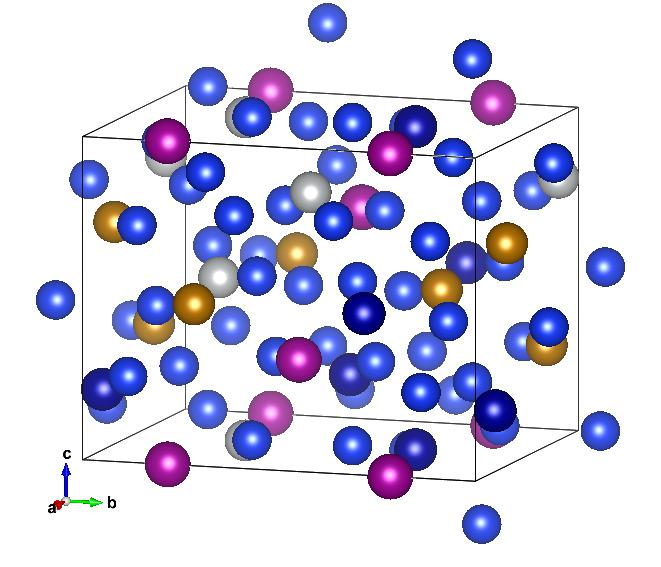
\includegraphics[width=\textwidth]{method/sqs/A.jpg}
\caption{Structure A}
\end{subfigure}
\hfill
\begin{subfigure}{0.5\textwidth}
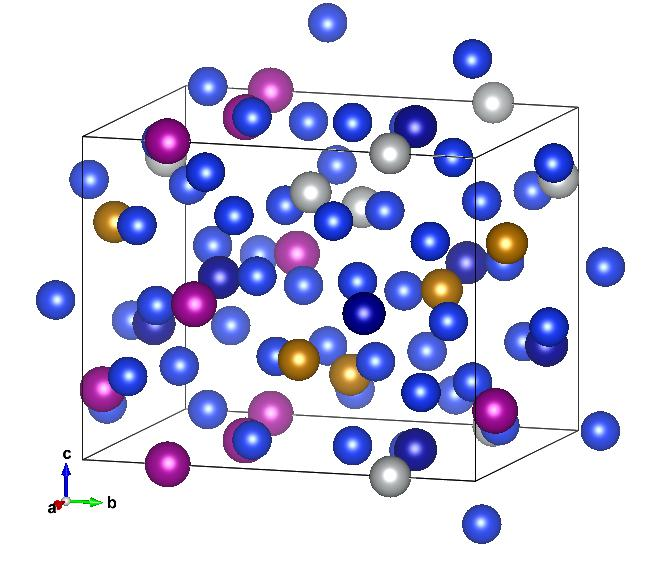
\includegraphics[width=\textwidth]{method/sqs/B.jpg}
\caption{Structure B}
\end{subfigure}
\begin{subfigure}{0.5\textwidth}
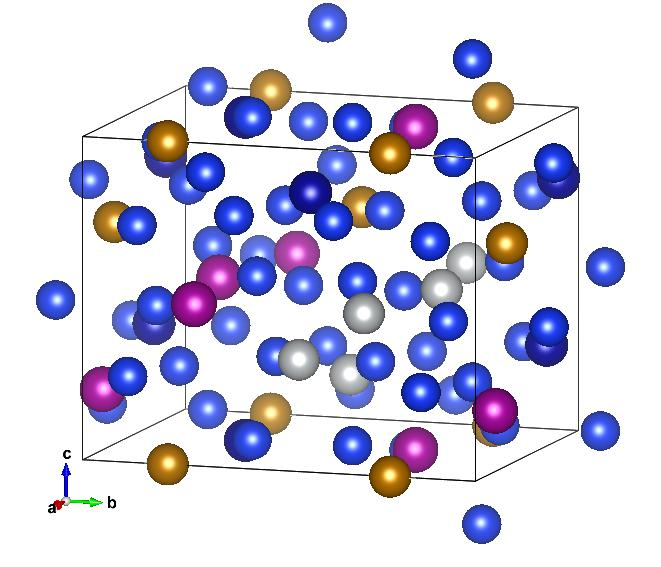
\includegraphics[width=\textwidth]{method/sqs/C.jpg}
\caption{Structure C}
\end{subfigure}
\hfill
\begin{subfigure}{0.5\textwidth}
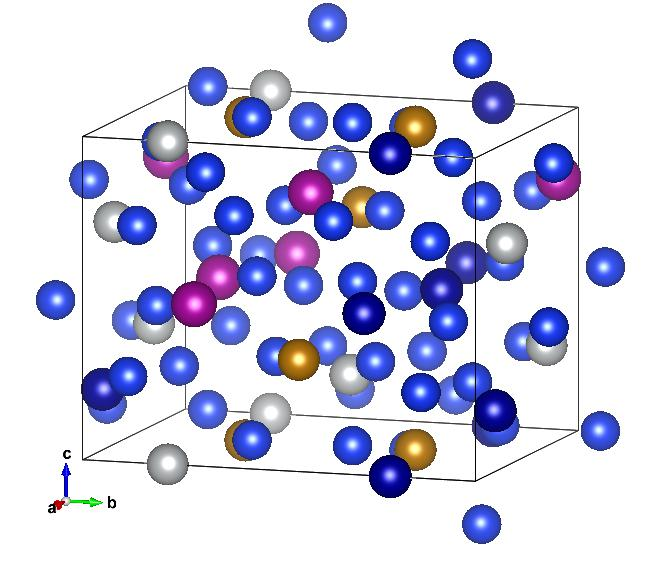
\includegraphics[width=\textwidth]{method/sqs/D.jpg}
\caption{Structure D}
\end{subfigure}
\begin{subfigure}{0.5\textwidth}
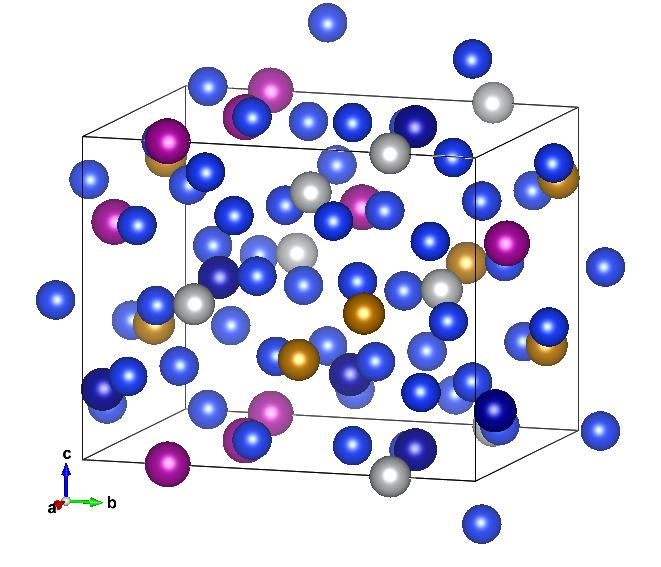
\includegraphics[width=\textwidth]{method/sqs/E.jpg}
\caption{Structure E}
\end{subfigure}
\caption{48 atom SQS based on eqvimolar distribution of Cr, Fe, Mn and Ni in and $FeSi_2$ cell.}
\label{sqs_FeSi2}
\end{figure}

\section{Band-structure?}

\section{Utility scripts}
During the course of the projects lifetime, several shell and python scripts was developed by myself and/or provided to me by my supervisor Ole Martin Løvvik and his team of researchers at Sintef. These can be located at the GitHub address :...
 mm  
\part{Results and Discussion}
\chapter{Working title}
\label{sec:something}


Throughout the duration of this study, we have carried out a great number of DFT calculations in order to present an comprehensive overview of promising high-entropy silicides. In payment to the thermoelectric prospect of hexagonal $Fe_2Si$, we firstly attempted to build SQSs from this structure. However, in agreement to the experimental indication that \textbf{cite?}, 3d silicides adopt a metallic character when the 3d elements supercede $50\%$ of the composition, all of our SQSs displayed a clear absence of an energy gap between the valence band and conduction band, we will return  more specifically to these compositions later in this section. For now, we will present the results of a much more interesting and promising case, in which we replaced $Fe_2Si$, with $\beta-FeSi_2$, effectively doubling the Si-metal ratio. Hence why we prefer the term high-entropy silicides more so than high-entropy alloys, as these particular compositions does not lie directly within the conditions presented in sections (\textbf{HEA}). In this structure, we completed in total calculations regarding 17 distinct compositions and permutations, such $\text{ALLOY}Si_2$ SQS based on CoCrFeni, CrFeMnNi, CoCrMnNi, CrFeMnTi, CrFeTiNi, and permutations wihin these such as increasing or decreasing the distribution of certain elements. Of the 17 variants, each consists of 5 unique SQSs, and trialed with numerous functionals, magnetic configurations and other parameters, as discussed in section .., in attempt to locate the overall most stable and reliable results. With this approach, the complete number of calculations and results both escalated very quikly, therefore, in the intent of presenting a clear and informative report of the study, we will begin this section by analyzing the overall most promising structure, then present and discuss these results in relation to the remaining permutations and structures.    

The aforementioned system is composed of Cr, Fe, Mn, and Ni, equally distributed in a 48 atom SQSs of $FeSi_2$, wheras 32 of these is silicon atoms. Here after, this system will be abbreviated CFMN (fesi2) to spcify that its within the framework of the cmce $FeSi_2$ unit cell.
 
The 5 distinct SQS can be seen in figure (method/SQS). Bellow, in table \ref{tab:FeSi2/CrFeMnNi_equal} we present a summary of the total energy, final magnetic moment and band gap corresponding to the 5 SQSs called A, B, C, D, and E respectfully. From a first glance, we observe very similar properties between the structures. The total energy per atom vary by $0.0092$ eV from the most stable structure C ($-6.6063$ eV) to the least stable structure D ($-6.6155$ eV). Similarly, the final magnetic moment is near identical throughout the span of SQSs, which is excepted given that aside from the unique distribution, all 5 SQSs contain the same amount and type of elements. On the contrary to the magnetic moment, the band gap is very sensitive to the type of SQS, ranging from a highest $0.05$ eV in structure B to $0$, ie nonexistent in structure D. A band gap in this range means for excellent application as thermoelectric materials. 


\begin{table}[H]
\centering
\begin{tabular}{@{}cccc@{}}
\toprule
Structure  & Total energy/atom (eV) & Final magnetic moment (?) & Band gap (eV) \\ \midrule
\textbf{A} & −6,6080                & 4.0006                    & 0.0280        \\
\textbf{B} & −6,6138                & 3.9999                    & 0.0523        \\
\textbf{C} & −6,6063                & 4.0008                    & 0.0344        \\
\textbf{D} & −6,6155                & 4.0001                    & 0             \\
\textbf{E} & −6,6089                & 4.0000                    & 0.0495        \\ \bottomrule
\end{tabular}
\caption{Total energy per atom, final magnetic moment, and band gap (GGA) of 5 $Cr_4Fe_4Mn_4Ni_4Si_{32}$ SQSs based on $FeSi_2$}
\label{table:fesi2_summary}
\end{table}  
Furthermore regarding the band gaps, we note that the gaps are indirect, the specific transitions is listed bellow.

\begin{table}[H]
\centering
\begin{tabular}{@{}ccc@{}}
\toprule
Structure  & Gap (D/I) & Transition                              \\ \midrule
\textbf{A} & I         & (0.500,0.333,0.500)-(0.500,0.000,0.000)  \\
\textbf{B} & I         & (0.250,0.000,0.250)-(0.000,0.000,0.000)  \\
\textbf{C} & -         & (0.500,0.000,0.500)-(-0.250,0.333,0.500) \\
\textbf{D} & I         & -                                        \\
\textbf{E} & I         & (0.000,0.000,0.000)-(0.250,0.000,0.250)  \\ \bottomrule
\end{tabular}
\caption{Band gap transition of CFMN (fesi2) SQSs with PBE functional}
\end{table}

In this regard, it would have been very instructive to plot a band structure diagram to further evaluate the energy bands, however due to the complex nature of the SQSs and the implementation with TDEP we were not able to plot the bandstructure. Thus, in this section we will analyze the band gap by other meassures. The first method we will employ is to observe the band gap from the plotted density of states, in figure \textbf{ref bellow}. From these figures, we can determine the band gap from the distance in energy around the Fermi energy (here set to 0), where the density of states is exactly 0, in addition we can observe the band gap for spin $\uparrow$ (positive) and $\downarrow$ (negative) states.   

\begin{figure}[H]
	\centering
	\begin{subfigure}{0.9\textwidth}
		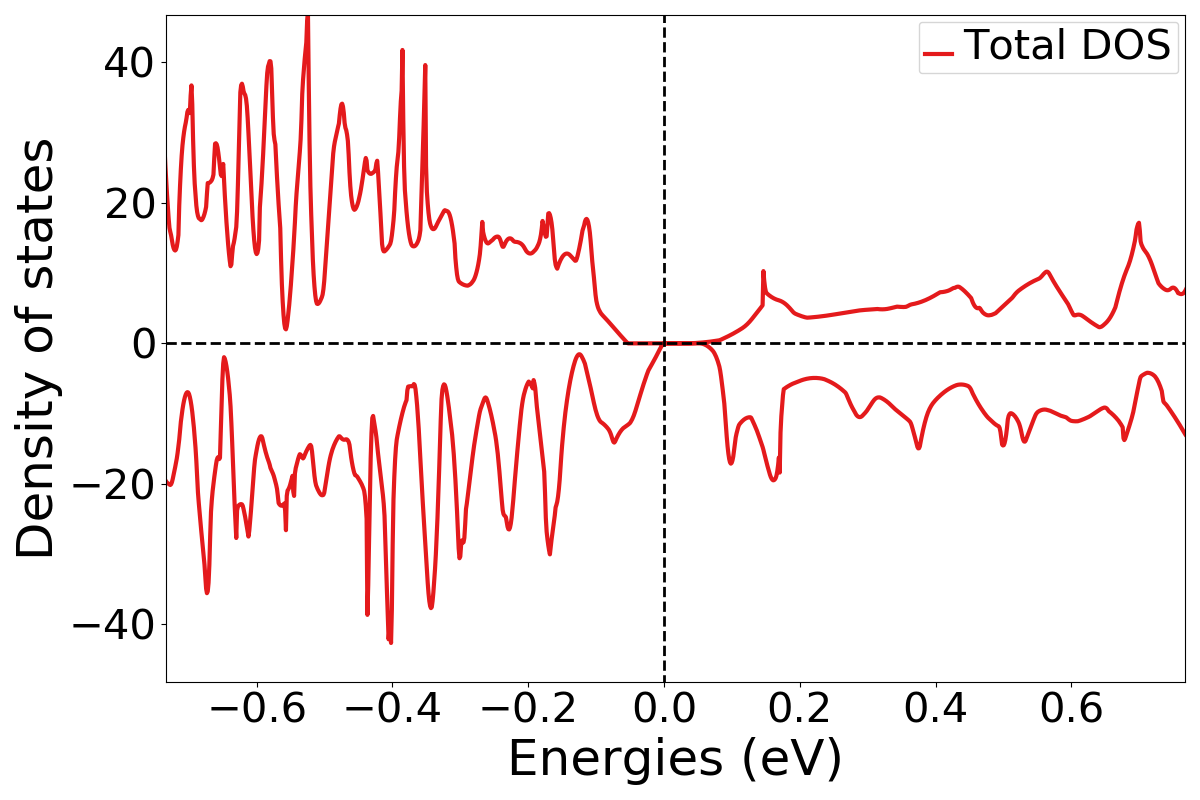
\includegraphics[width=\textwidth]{results/fesi2/DOS_A_toten.png}
	\end{subfigure}

	\begin{subfigure}{0.9\textwidth}
		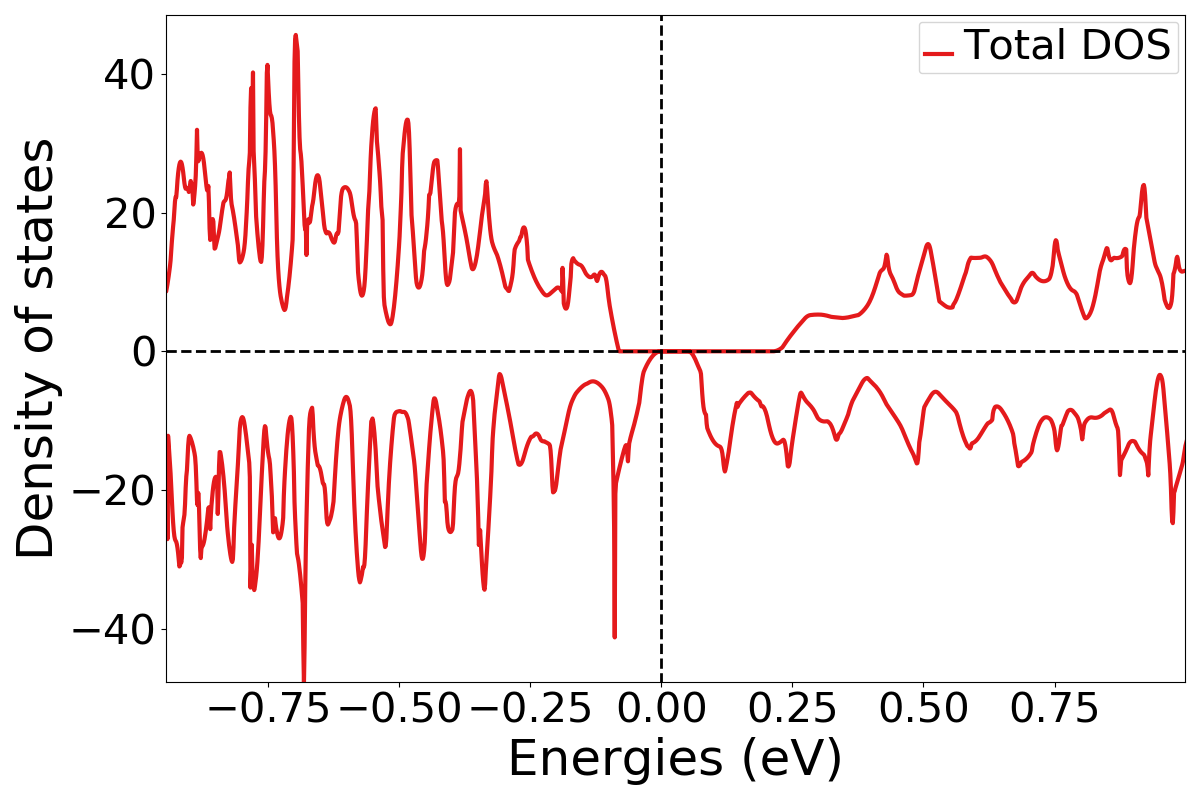
\includegraphics[width=\textwidth]{results/fesi2/DOS_B_toten.png}
	\end{subfigure}
	\begin{subfigure}{0.9\textwidth}
		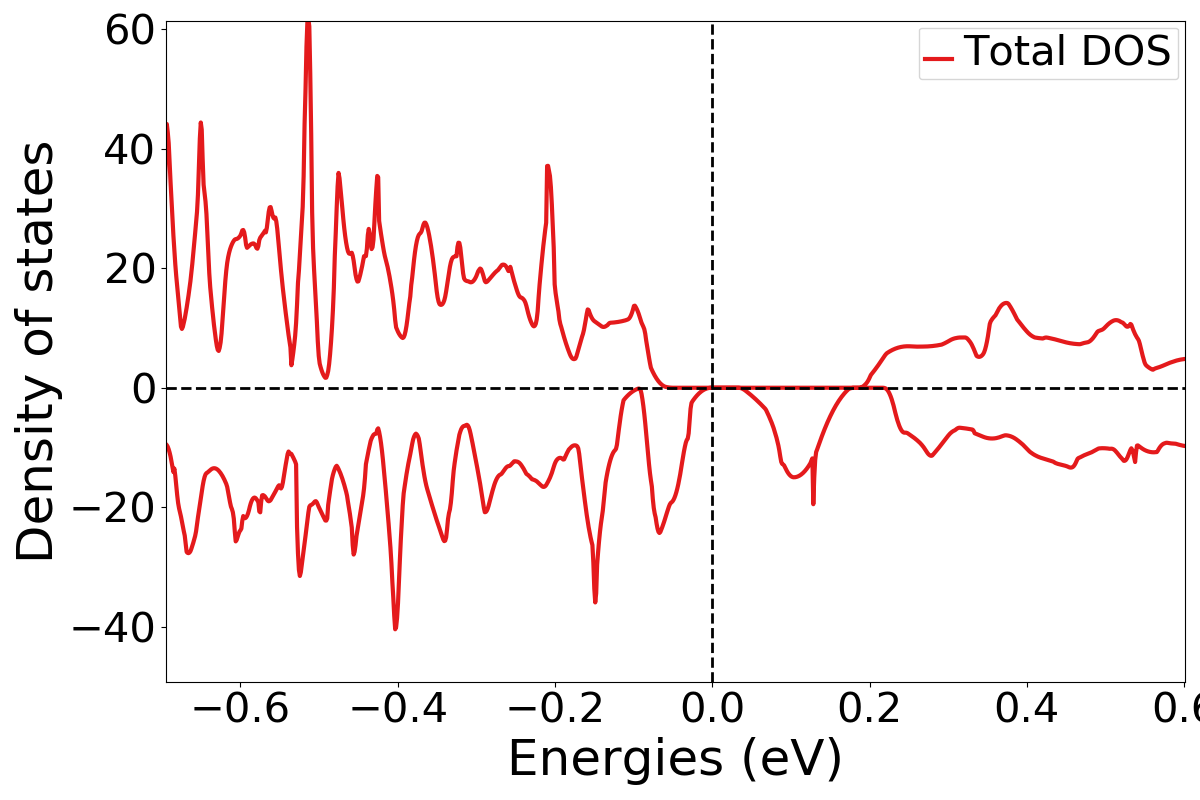
\includegraphics[width=\textwidth]{results/fesi2/DOS_C_toten.png}
	\end{subfigure}
\end{figure}
\begin{figure}[H]
	\centering
	\begin{subfigure}{0.9\textwidth}
		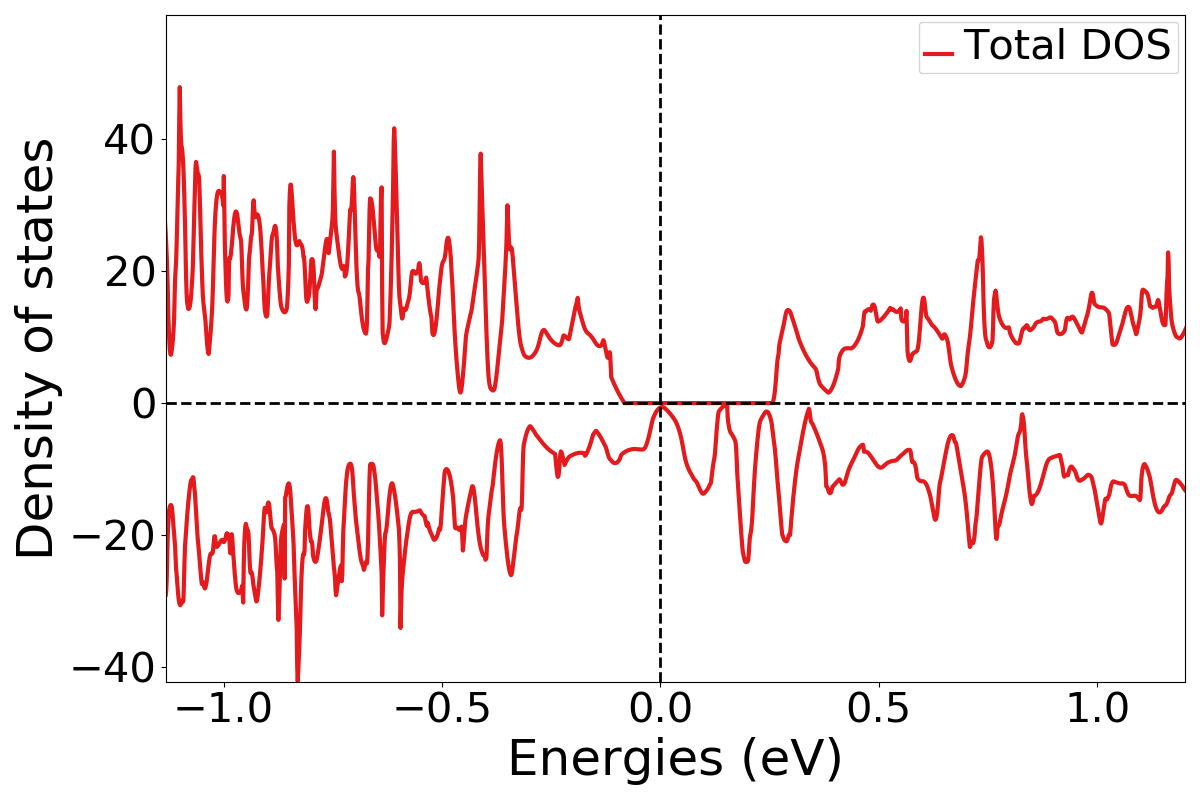
\includegraphics[width=\textwidth]{results/fesi2/DOS_D_toten.png}
	\end{subfigure}
	\begin{subfigure}{0.9\textwidth}
		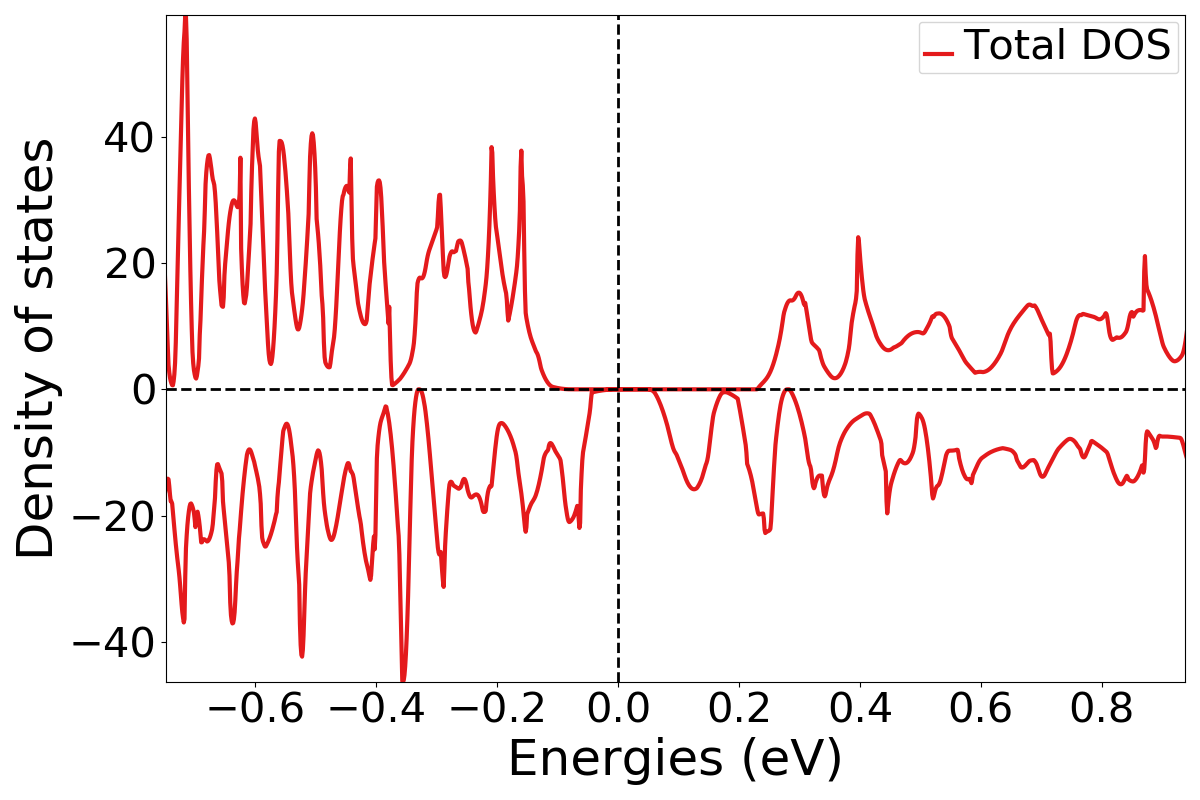
\includegraphics[width=\textwidth]{results/fesi2/DOS_E_toten.png}
	\end{subfigure}
	\caption{Density of states for structure A, B, C, D, E of $CFMNSi_2 (FeSi_2)$ SQSs (PBE GGA)}
	\label{dos_fesi2_gga}
\end{figure}



\begin{comment}
\begin{table}[H]
\centering
\begin{tabular}{@{}cccc@{}}
\toprule
Structure  & Spin-up & Spin-down & Total  \\ \midrule
\textbf{A} & 0.0814  & 0.0522    & 0.0281 \\
\textbf{B} & 0.2932  & 0.0523    & 0.0523 \\
\textbf{C} & 0.2355  & 0.0343    & 0.0343 \\
\textbf{D} & 0.3386  & 0         & 0      \\
\textbf{E} & 0.3078  & 0.0495    & 0.0495 \\ \bottomrule
\end{tabular}
\caption{Band gap (GGA) in spin up and spin down channels of CFMNSi2 structures}
\end{table}

\begin{table}[H]
\centering
\begin{tabular}{@{}cccc@{}}
\toprule
Structure  & PBE    & SCAN   & HSE06  \\ \midrule
\textbf{A} & 0.0281 & 0.0000 & 0.0207 \\
\textbf{B} & 0.0523 & 0.0890 & 0.1808 \\
\textbf{C} & 0.0344 & 0.0690 & 0.0196 \\
\textbf{D} & 0.0000 & 0.0000 & 0.0000 \\
\textbf{E} & 0.0495 & 0.1048 & 0.0133 \\ \bottomrule
\end{tabular}
\caption{Band gap of $CFMN (FeSi_2)$ SQSs with GGA (PBE), meta-GGA (SCAN) and hybrid-functionals (HSE06). \textbf{Add footnote to explain the uncertainty in these results regarding smearing type and width, and DOS and EIGENVAL}}
\end{table}
\end{comment}

\textbf{DOS analyse}

\begin{figure}[H]
\centering
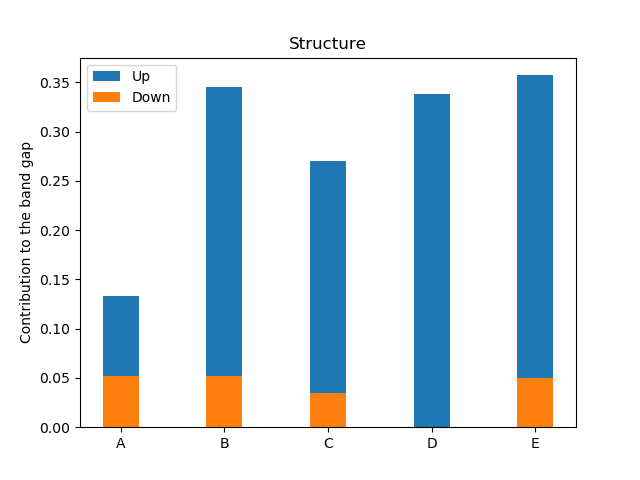
\includegraphics[scale=.7]{results/fesi2/spin_gap.png}
\caption{Band gap of CFMN fesi2 SQSs in spin up and spin down with PBE functional.}
\label{DOS_hse06_B}
\end{figure}

\textbf{Intro LDOS}

\textbf{Diskusjon LDOS}

\begin{figure}[H]
%\centering
	\begin{subfigure}{\textwidth}
		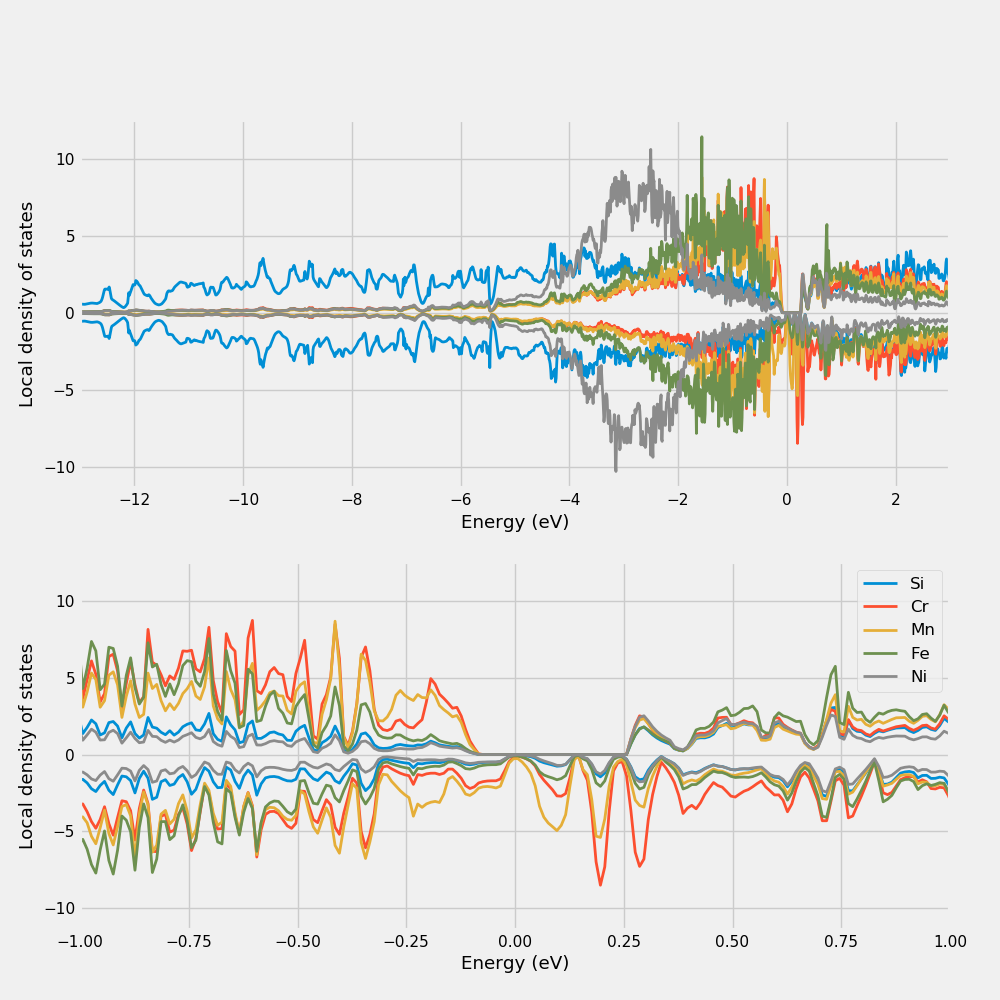
\includegraphics[width=\textwidth]{results/fesi2/A_LDOS.png}
		\caption{A}
	\end{subfigure}
	\begin{subfigure}{\textwidth}
		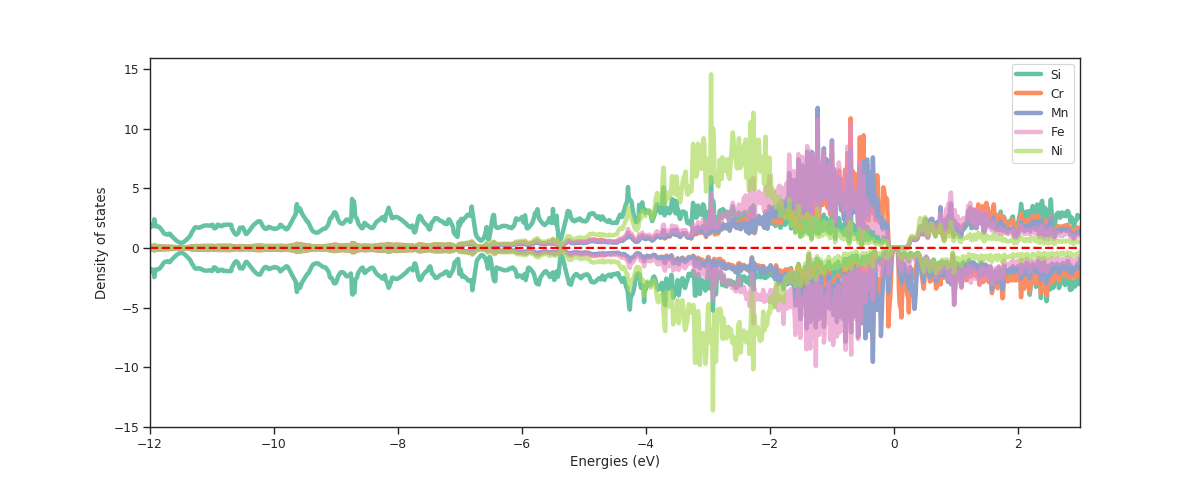
\includegraphics[width=\textwidth]{results/fesi2/B_LDOS.png}
		\caption{B}
	\end{subfigure}
	\begin{subfigure}{\textwidth}
		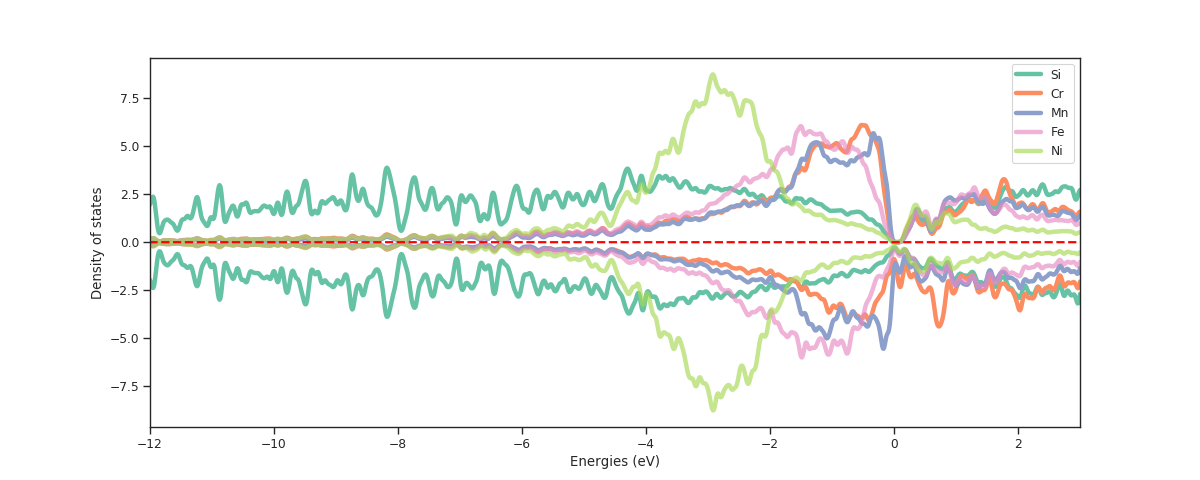
\includegraphics[width=\textwidth]{results/fesi2/C_LDOS.png}
		\caption{C}
	\end{subfigure}
	\begin{subfigure}{\textwidth}
		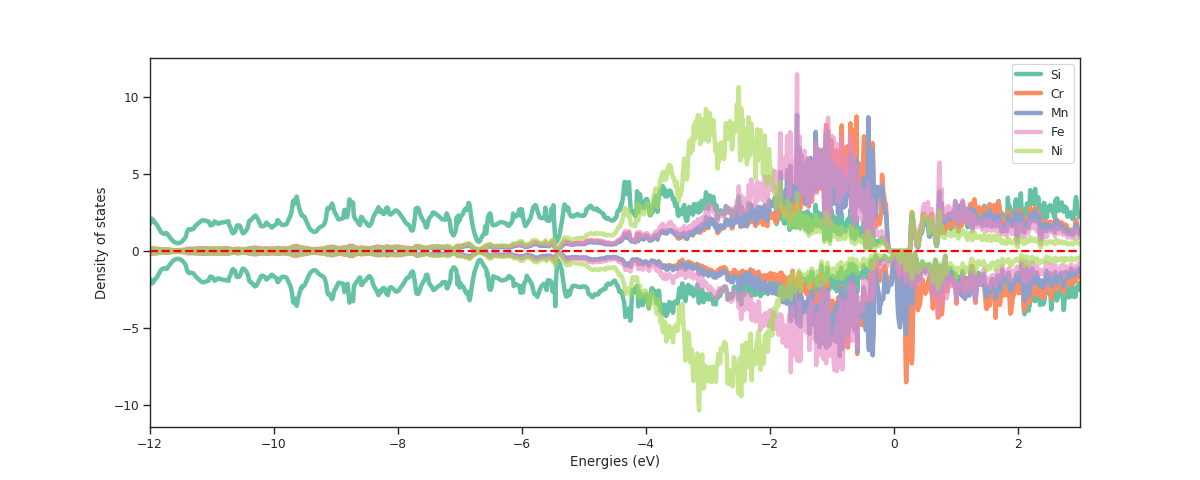
\includegraphics[width=\textwidth]{results/fesi2/D_LDOS.png}
		\caption{D}
	\end{subfigure}
\end{figure}		
\begin{figure}[H]
	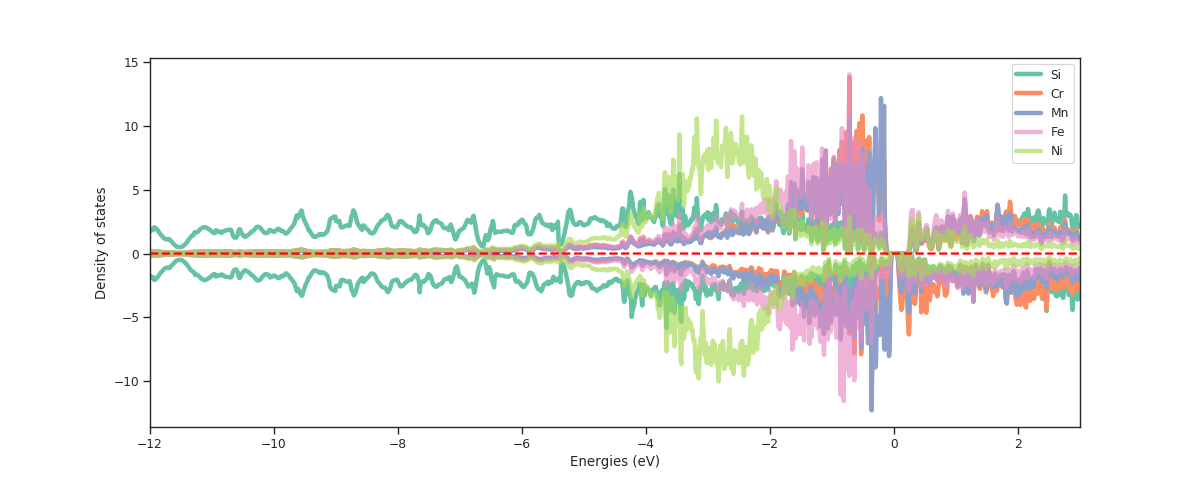
\includegraphics[width=\textwidth]{results/fesi2/E_LDOS.png}
	\caption{E}
\end{figure}

\textbf{Continue discussion LDOS, introduce and discuss PDFs}

\begin{figure}[H]
%\centering
	\begin{subfigure}{\textwidth}
		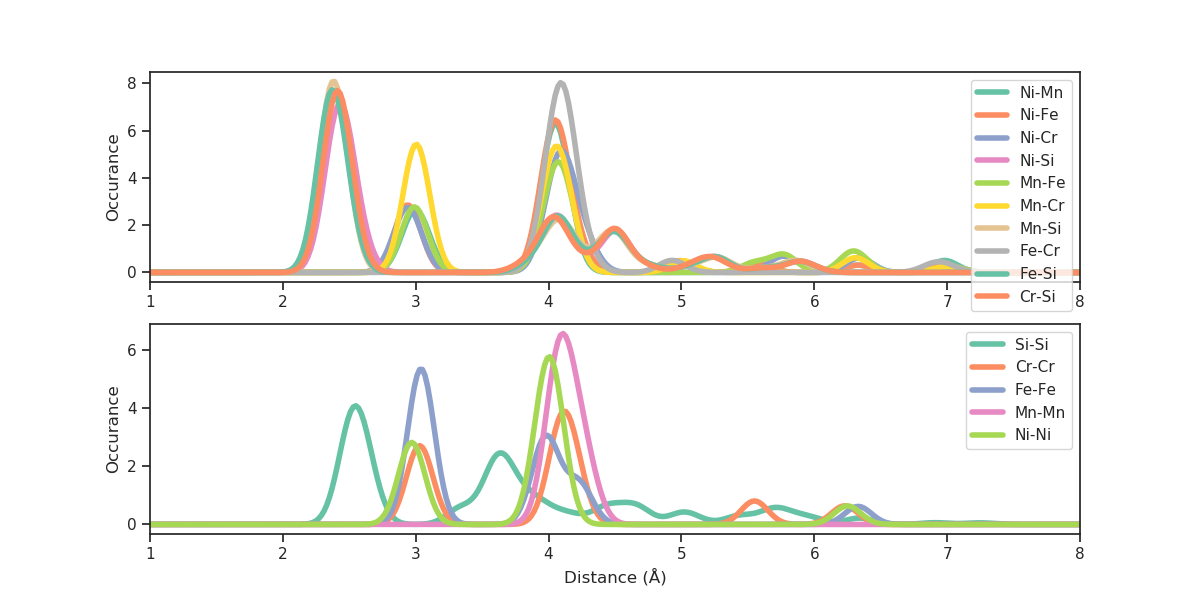
\includegraphics[width=\textwidth]{results/fesi2/A_PDF.png}
		\subcaption{A}
	\end{subfigure}	
	\begin{subfigure}{\textwidth}
		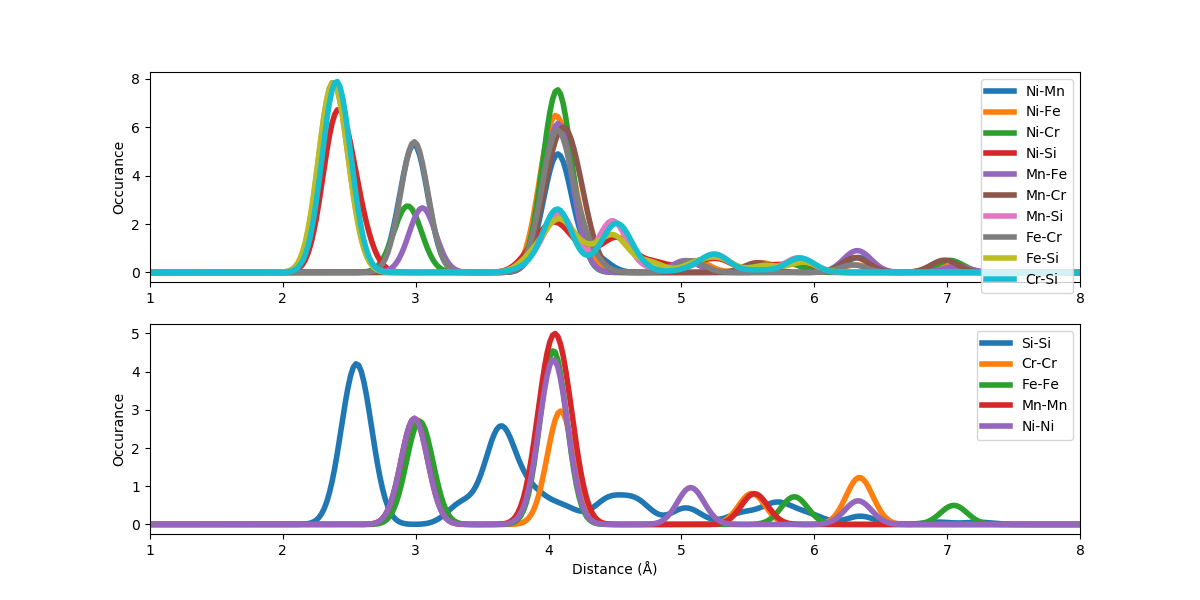
\includegraphics[width=\textwidth]{results/fesi2/B_PDF.png}
		\subcaption{B}
	\end{subfigure}
	\begin{subfigure}{\textwidth}
		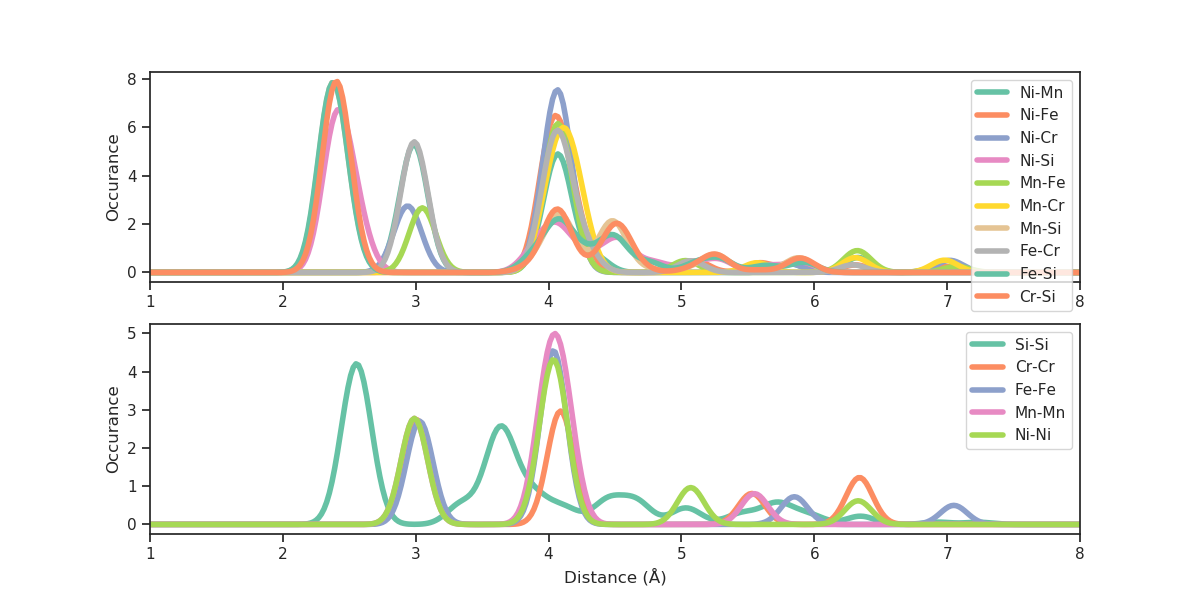
\includegraphics[width=\textwidth]{results/fesi2/C_PDF.png}
		\subcaption{C}
	\end{subfigure}
\end{figure}
\begin{figure}[H]
	\begin{subfigure}{\textwidth}
		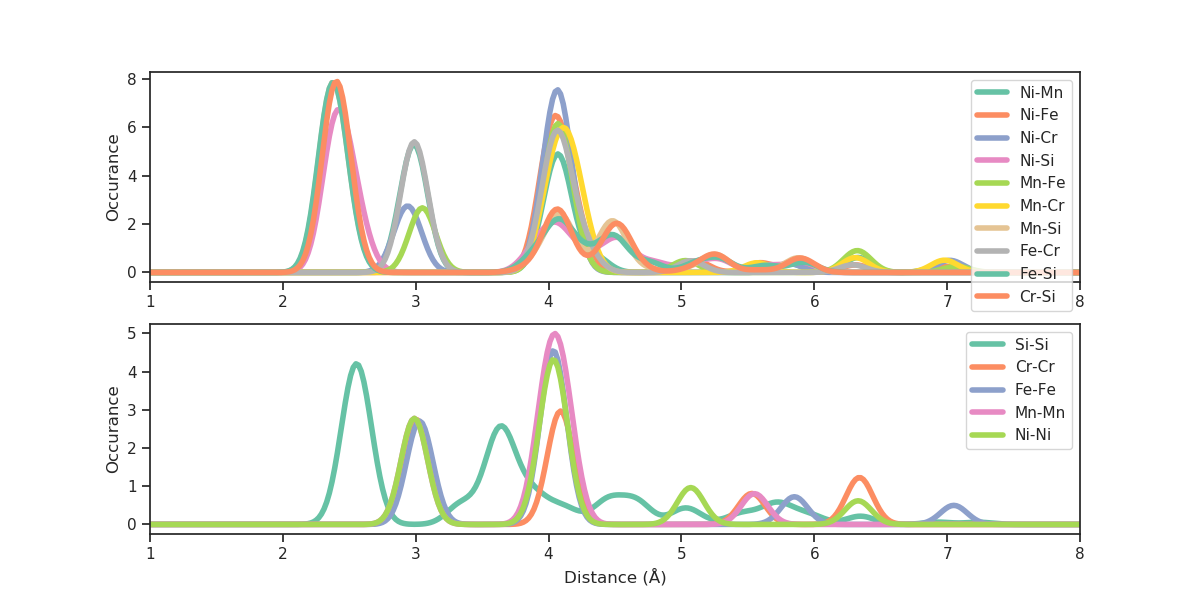
\includegraphics[width=\textwidth]{results/fesi2/D_PDF.png}
		\subcaption{D}
	\end{subfigure}
	\begin{subfigure}{\textwidth}
		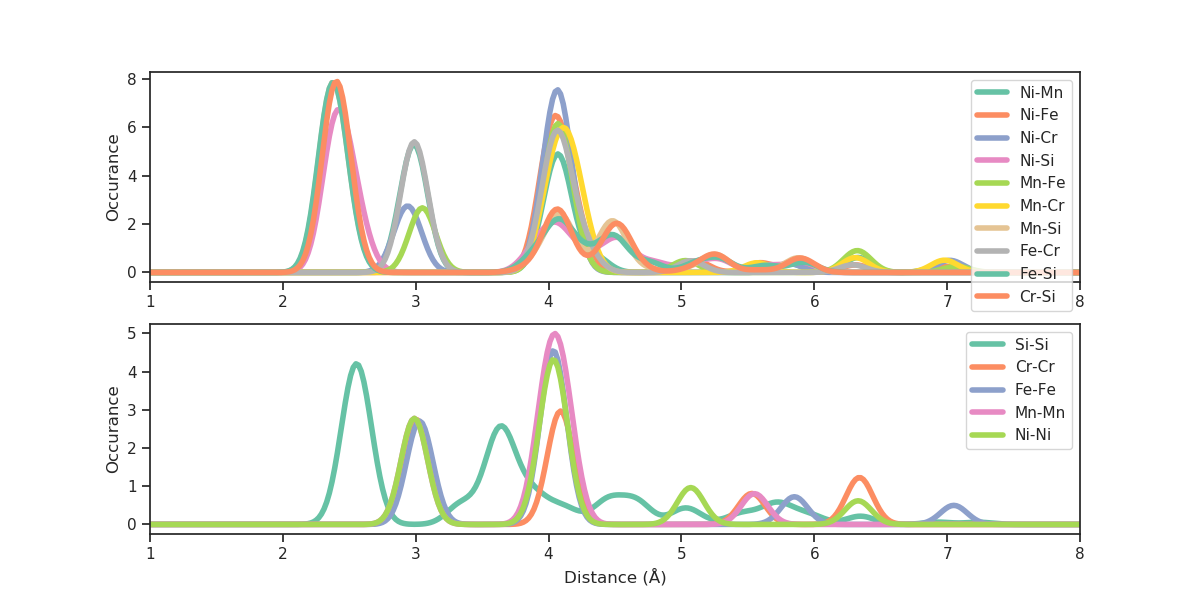
\includegraphics[width=\textwidth]{results/fesi2/E_PDF.png}
		\subcaption{E}
	\end{subfigure}
\end{figure}

\textbf{Finish discussion pdfs, introduce CHGCAR}

\begin{figure}
	\begin{subfigure}{0.5\textwidth}
		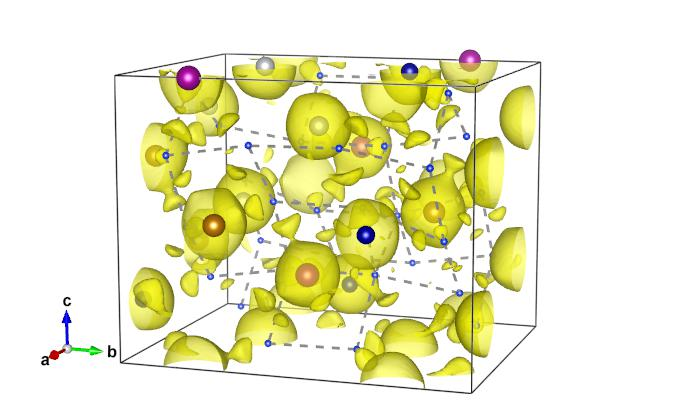
\includegraphics[width=\textwidth]{results/fesi2/A_CHGCAR.jpg}
		\caption{Structure A}
	\end{subfigure}
	\hfill
	\begin{subfigure}{0.5\textwidth}
		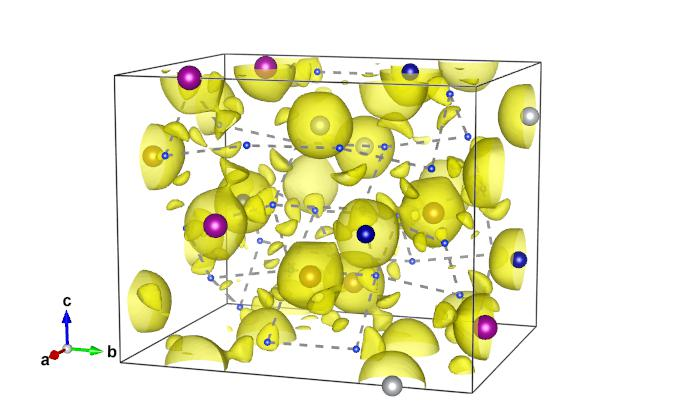
\includegraphics[width=\textwidth]{results/fesi2/B_CHGCAR.jpg}
		\caption{Structure B}
	\end{subfigure}
	\begin{subfigure}{0.5\textwidth}
		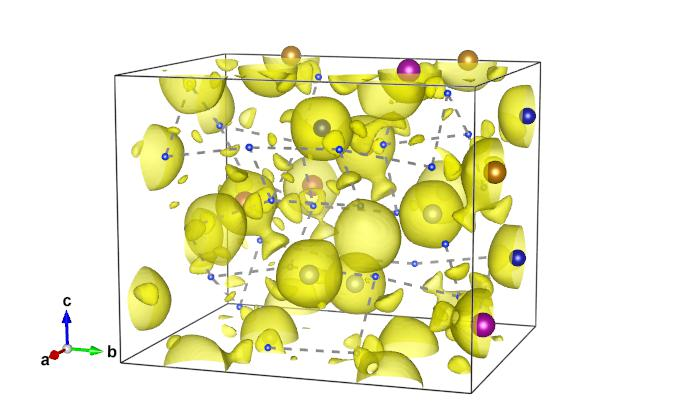
\includegraphics[width=\textwidth]{results/fesi2/C_CHGCAR.jpg}
		\caption{Structure C}
	\end{subfigure}
	\hfill
	\begin{subfigure}{0.5\textwidth}
		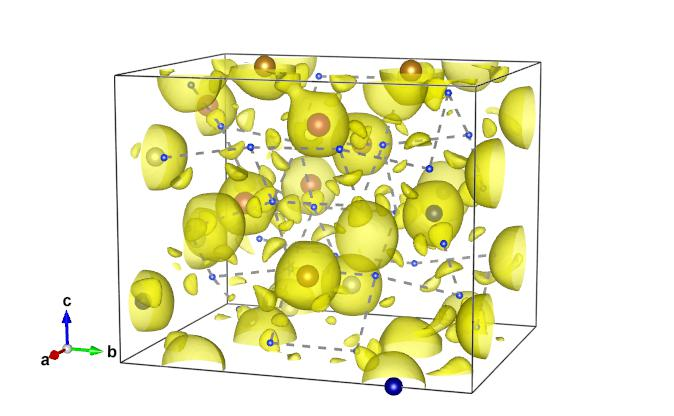
\includegraphics[width=\textwidth]{results/fesi2/D_CHGCAR.jpg}
		\caption{Structure D}
	\end{subfigure}
	\begin{subfigure}{0.5\textwidth}
		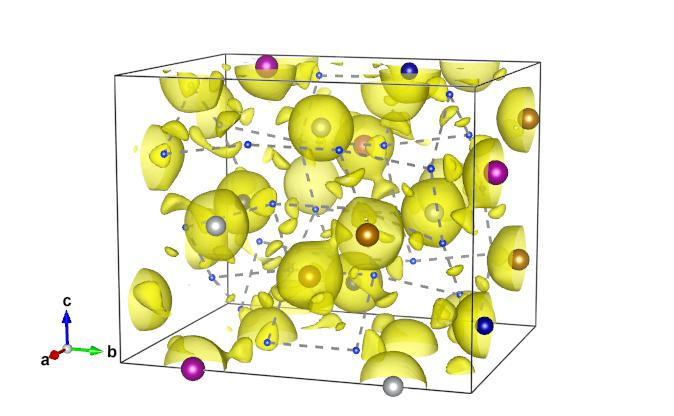
\includegraphics[width=\textwidth]{results/fesi2/E_CHGCAR.jpg}
		\caption{Structure E}
	\end{subfigure}
		\caption{Charge density}
		\label{chgcar}
\end{figure}



\textbf{Discuss CHGCAR and summarize/conclude this section. Include aspects such as stability and magnetic configuration, important here to draw parallels and discuss the results in light of high-entropy alloys, SQS, DFT and thermoelectricity. }

\textbf{Transistion into other methods and structures, present first results from SCAN and HSE06 for these 5 structures, discuss these results, but to lesser detail than PBE section. Then when finished with that, present, briefly discuss and summarize the results from all remaining structures, only include figures with good results, maybe others as well for the sake of comparison. The remaining data can be easily included in either the appendix or in a tabular format. }

\begin{figure}[H]
\centering
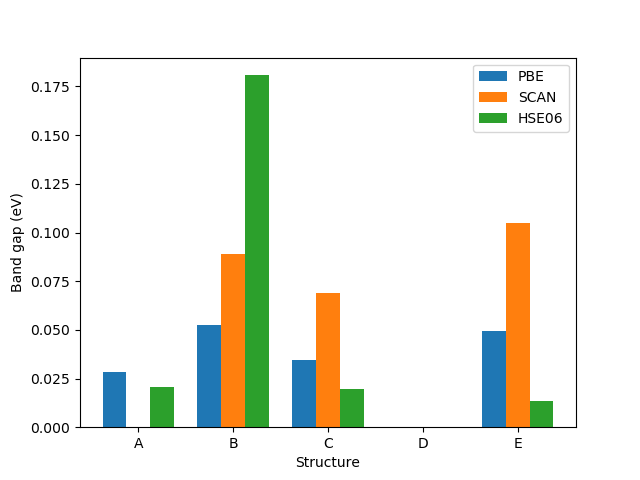
\includegraphics[scale=.7]{results/fesi2/xc_gap.png}
\caption{Band gap of CFMN (fesi2) all 5 SQSs with PBE, SCAN and HSE06}
\label{Xc_fig}
\end{figure}


Looking at the results from different functionals, we observe that the hybrid functional HSE06 more or less agree with results of the PBE functional in terms of the actual presence of the band gap, while the size of the gap is up for debate. Especially in B, where we observe a band gap greater than 0.18 eV in comparison to 0.05 eV with PBE and 0.08 with SCAN. Bellow we show the total density of states around the fermi energi $E_f$ for this structure with the HSE06 functional. 

\begin{figure}[H]
\centering
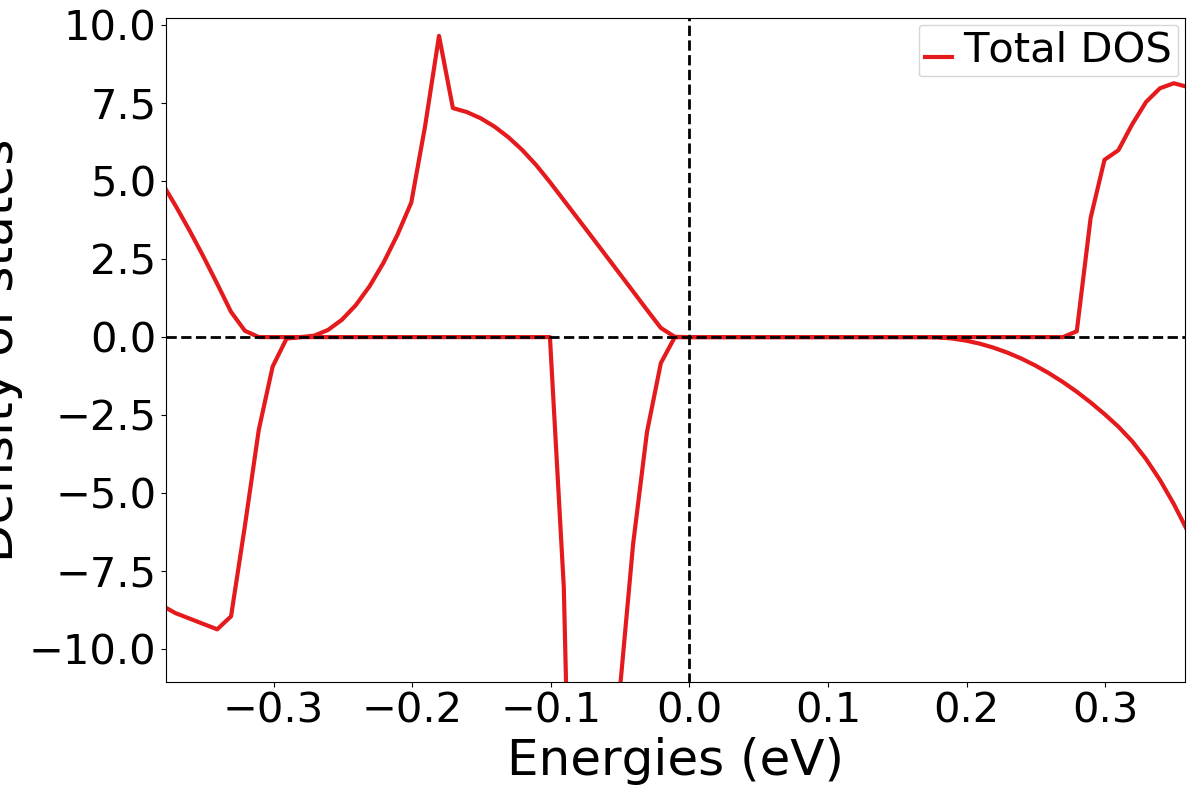
\includegraphics[scale=.3]{results/fesi2/hse06/B_DOS_zoom.png}
\caption{Density of states from HSE06 of $FeSi_2$ CFMN structure B}
\label{DOS_hse06_B}
\end{figure}

If we now compare this to the density of states of structure E,

\begin{figure}[H]
%\centering
\begin{subfigure}{0.5\textwidth}
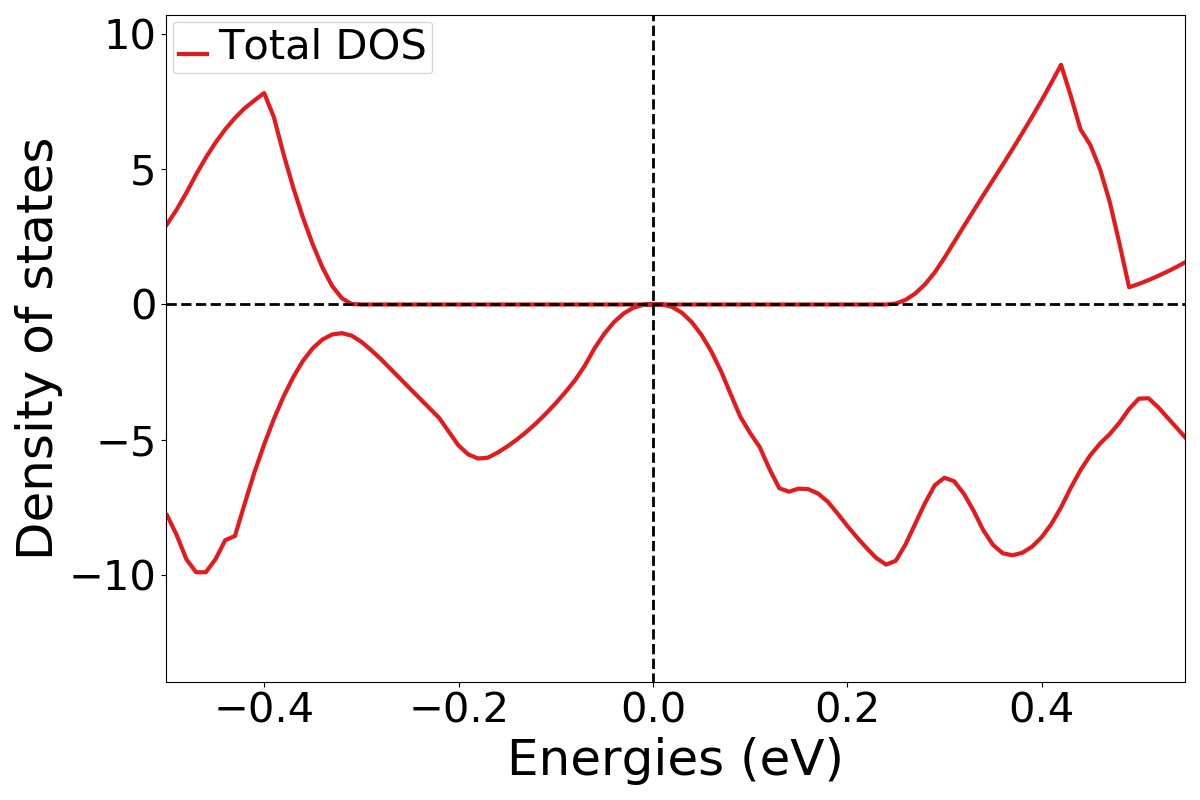
\includegraphics[width=\textwidth]{results/fesi2/hse06/E_DOS_zoom.png}
\caption{DOS $\uparrow, \downarrow$}
\end{subfigure}
\hfill
\begin{subfigure}{0.5\textwidth}
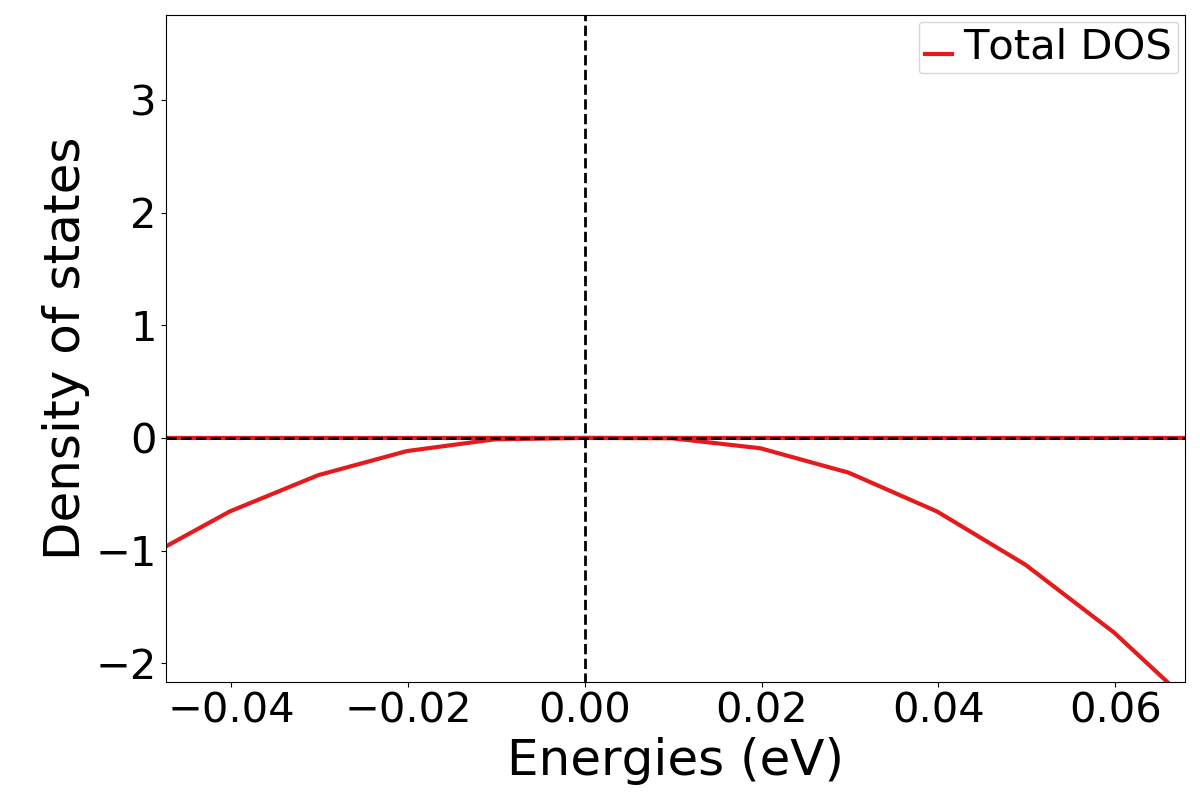
\includegraphics[width=\textwidth]{results/fesi2/hse06/E_DOS_down.png}
\caption{DOS $\downarrow$}
\end{subfigure}
\caption{The density of states of CFMN ($FeSi_2$) structure E for a) spin up and down, and b) focused on spin down}
\end{figure}


\textbf{I think its relevant and interesting to in-depth analyze structure B, D, and E. B because of large band gap. D because no band gap, and E because this well represents the other structures A and C. }
One difference is the KS eigenvalues. Str D have both partial occupancy and nonphysical occupancy, ie above 1 and bellow zero both in PBE and HSE06. This is not the case for structures that exhibited band gaps. Here we have clear transition from 1 to 0. Without having done a broad investigation of all material. This seems to be the case in other compositions and cells and permutations as well. Where both partial occupants and nonphysical occupations result in metallic structures. Calculating the band gap with strict 1 and 0 conditions, lead to small band gaps in most structures. Furthermore, in structures of Fe2Si, the difference in band where occupation transition from 1 to 0 between up and down, increases hugely compared to FeSi2 structures, talking close to 20 bands, opposed to maybe 2-5. 


\part{Conclusion}

\backmatter{}
\printbibliography
\end{document}
